% Define the document style. The thesis stylesheet inherits from 'report'. 
% I had once made a version inheriting from book. However the two versions are almost 
% compatible. The main difference is that the other version supported 'parts'.
% (extended from book) and this does not.
% IST requires the thesis to be written in Arial or similar. Two arguments allow you 
% to define the thesis font: 'Helvetica' and 'AvantGarde', which transforms normal font
% into Helvetica or AvantGarde, respectively... dahhhh!
\documentclass[defaultstyle,10pt,a4paper,master,Helvetica]{thesis}
%\documentclass[defaultstyle,12pt,phd]{thesis}

% Defines an additional alphabet... not required in most cases
% ------------------------------------------------------------
% \DeclareMathAlphabet{\mathpzc}{OT1}{pzc}{m}{it}

% PACKAGE fontenc:
% -----------------
% chooses T1-fonts and allows correct automatic hyphenation.
\usepackage[T1]{fontenc}
\usepackage[latin1]{inputenc}

% PACKAGE babel:
% ---------------
% The 'babel' package may correct some hyphenisation issues of latex. 
% However in most situations it is not required.
\usepackage[portuges]{babel}

% PACKAGE latexsym:
% -----------------
% Defines additional latex symbols. May be required for thesis with many math symbols.
%\usepackage{latexsym}

% PACKAGE amsmath, amsthm, amssymb, amsfonts:
% -------------------------------------------
% This package is typically required. Among many other things it adds the possibility
% to put symbols in bold by using \boldsymbol (not \mathbf); defines additional 
% fonts and symbols; adds the \eqref command for citing equations. I prefer the style
% "(x.xx)" for referering to an equation than to use "equation x.xx".
\usepackage{amsmath, amsthm, amssymb, amsfonts}

% PACKAGE multirow, colortbl, longtable:
% ---------------------------------------
% These packages are most usefull for advanced tables. The first allows to join rows 
% throuhg the command \multirow which works similarly with the command \multicolumn
% The second package allows to color the table (both foreground and background)
% The third package is only required when tables extend beyond the length of one page;
% which typically does not happen and should be avoided
\usepackage{multirow}
\usepackage{colortbl}
% \usepackage{longtable}

% PACKAGE graphics, epsfig, subfigure, caption:
% ---------------------------------------------
% Packages for figures... well you will certainly need these packages, with the exception
% of the 'caption' package. This only allows to define extra caption options.
% Notice that subfigure allows to place figures within figures with its own caption. It
% should be avoided to create an eps file with subfigures. That will mean that you won't be 
% able to reference those subfigures. Instead create an EPS file (the only graphics format supported
% by latex) for each of the subfigures and then use the command \subfigure (see below).
\usepackage{graphicx}
\usepackage{epsfig}
\usepackage[hang,small,bf]{subfigure}
% \usepackage[hang,small,bf]{caption}

% PACKAGE algorithmic, algorithm
% ------------------------------
% These packages are required if you need to describe an algorithm.
% \usepackage{algorithmic}
% \usepackage[chapter]{algorithm}

% PACKAGE natbib/cite
% -------------------
% The two packages are not compatible, and you should use one of the two. Notice however that the
% IEEE BiBTeX stylesheet is imcompatible with the natbib package. If using the IEEE format, use the 
% cite package instead
\usepackage[square,numbers,sort&compress]{natbib}
%\usepackage{cite}

% PACKAGE acronyum
% -----------------
% This package is most usefull for acronyms. The package garantees that all acronyms definitions are 
% given at the first usage. IMPORTANT: do not use acronyms in titles/captions; otherwise the definition 
% will appear on the table of contents.
\usepackage[printonlyused,withpage]{acronym}

% PACKAGE extra_functions
% -----------------
% My Personal package: defines the following commands:
% \fancychapter{chaptername) -> Prints a fancier chapter (you can also use the fancychapter package for this)
% \hline{width} -> use for a replacement of the \hline command
% \Mark1, \Mark2, \Mark3, ...
\usepackage{extra_functions}

% PACKAGE tocloft
% -----------------
% The tocloft package provides means of controlling the typographic design of the Table of Contents,
% List of Figures and List of Tables. New kinds of `List of . . . ' can be defined.
% The package has been tested with the tocbibind, minitoc, ccaption, subfigure, float, fncychap, and hyperref packages.
\usepackage[subfigure]{tocloft}

% PACKAGE babelbib
% -----------------
\usepackage[fixlanguage]{babelbib}
\selectbiblanguage{portuges}

% PACKAGE todonotes
% -----------------
% \usepackage{todonotes}

% PACKAGE IEEEtrantools
% -----------------
% Allows customization of the IEEEtran bibliography style
% \usepackage[retainorgcmds]{IEEEtrantools}

% PACKAGE fixltx2e
% -----------------
% Allows the \textsubscript{} command, among other fixes
\usepackage{fixltx2e}

% PACKAGE longtable
% -----------------
% Use this instead of tabular when you need footnotes inside a table
\usepackage{longtable}

% PACKAGE hyperref
% -----------------
% Set links for references and citations in document
% Some MiKTeX distributions have faulty PDF creators in which case this package will not work correctly
% Long live Linux :D
\usepackage{hyperref}
\hypersetup{ a4paper=true,
             colorlinks=false,
             citecolor=red,
             breaklinks=true,
%            bookmarks=true,		% commented because it generated a warning
             bookmarksnumbered=true,
             bookmarksopen=true,
             pdftitle={T�tulo do PDF},
             pdfauthor={Autor},
             pdfsubject={Tese de Mestrado},
             pdfcreator={LaTeX},
             pdfkeywords={}
}

\def\chapterautorefname{Cap�tulo}
\def\sectionautorefname{Sec��o}
\def\subsectionautorefname{Subsec��o}
\def\figureautorefname{Figura}
\def\tableautorefname{Tabela}

% PACKAGE hypcap
% -----------------
% In case you use the package hyperref to create a PDF, the links to tables or figures
% will point to the caption of the table or figure, which is always below the table or figure itself.
% Therefore the table or figure will not be visible, it is above the pointer and one has
% to scroll up in order to see it.
% If you want the link point to the top of the image you can use this package
\usepackage[all]{hypcap}

% PACKAGE breakurl
% -----------------
% Provides breakable URLs
% This package is designed to be loaded after hyperref to provide a breakable
% hyperlinked \url command under DVI output
%
% Note: apparently not needed when using pdfTeX
% \usepackage{breakurl}

% Set paragraph counter to alphanumeric mode
\renewcommand{\theparagraph}{\Alph{paragraph}~--}

% Page formatting... It was correct for my master thesis... not sure it is still correct
\hoffset 0in
\voffset 0in
\oddsidemargin 0.71cm
\evensidemargin 0.04cm
\marginparsep 0in
\topmargin -0.25cm
\textwidth 15cm
\textheight 23.5cm

\usepackage{fancyhdr}
\pagestyle{fancy}
\renewcommand{\chaptermark}[1]{\markboth{\thechapter.\ #1}{}}
\renewcommand{\sectionmark}[1]{\markright{\thesection\ #1}}
\fancyhf{} \fancyhead[LE]{\bfseries\nouppercase{\leftmark}}
\fancyhead[RO]{\bfseries\nouppercase{\rightmark}}
\fancyfoot[LE,RO]{\bfseries\thepage}
\renewcommand{\headrulewidth}{0.5pt}
\renewcommand{\footrulewidth}{0.5pt}
\addtolength{\headheight}{2pt} % make space for the rule
\fancypagestyle{plain}{%
   \fancyhead{} % get rid of headers
   \renewcommand{\headrulewidth}{0pt} % and the line
   \renewcommand{\footrulewidth}{0pt}
}
\fancypagestyle{blank}{%
   \fancyhf{} % get rid of headers and footers
   \renewcommand{\headrulewidth}{0pt} % and the line
   \renewcommand{\footrulewidth}{0pt}
}
\fancypagestyle{abstract}{%
   \fancyhead{}
   \renewcommand{\headrulewidth}{0pt}
   \renewcommand{\footrulewidth}{0.5pt}
}
\fancypagestyle{document}{%
	\fancyhf{} \fancyhead[LE]{\bfseries\nouppercase{\leftmark}}
	\fancyhead[RO]{\bfseries\nouppercase{\rightmark}}
	\fancyfoot[LE,RO]{\bfseries\thepage}
	\renewcommand{\headrulewidth}{0.5pt}
	\renewcommand{\footrulewidth}{0.5pt}
	\addtolength{\headheight}{2pt} % make space for the rule
}
\setcounter{secnumdepth} {5}
\setcounter{tocdepth} {5}
\renewcommand{\thesubsubsection}{\thesubsection.\Alph{subsubsection}}

\renewcommand{\subfigtopskip}{0.3 cm}
\renewcommand{\subfigbottomskip}{0.2 cm}
\renewcommand{\subfigcapskip}{0.3 cm}
\renewcommand{\subfigcapmargin}{0.2 cm}


% Custom commands for automatic text
% (remember to add {} after each one, or adjacent spaces will be suppressed)
\newcommand{\isocless}{\mbox{ISO/IEC 14443}}
\newcommand{\extlog}{\textit{Extended Logging}}
\newcommand{\emv}{\nameref{sec:ea:emv}}

\newcommand{\acroemph}[1]{\textit{#1}}

\begin{document}

% This solves a pdfTeX warning about page counters related to hyperref
% See: http://en.wikibooks.org/wiki/LaTeX/Packages/Hyperref#Problems_with_Links
\pagenumbering{alph}

% Add PDF bookmark 
\pdfbookmark[0]{Capa}{Titlepage}

%%%%%%%%%%%%%%%%%%%%%%%%%%%%%%%%%%%%%%%%%%%%%%%%%%%%%%%%%%%%%%%%%%%%%%%%%%%%%%%%%%%%%%%%%%%%%%%%
% DEFINE THE TITLEPAGE
% remember that IST requires for the titlepage to be written in portuguese
%%%%%%%%%%%%%%%%%%%%%%%%%%%%%%%%%%%%%%%%%%%%%%%%%%%%%%%%%%%%%%%%%%%%%%%%%%%%%%%%%%%%%%%%%%%%%%%%
% REQUIRED:
% The university logo image: first and second arguments are the (top,left) position of the logo. 
% IST rules force it to be 2cm
\univlogo{3cm}{2cm}{pdf/0_logo_ist_web.pdf}
% OPTIONAL:
% The thesis logo image: first and second arguments are the position of the logo. 
%\thesislogo{2.5cm}{6cm}{img/0_cover_image.png}

% Thesis title
\title{Monitoriza��o Wireless de Pessoas em Ambiente Dom�stico}

% Author and highest current degree (not the one you are applying to)
\author{M�rcio Lu�s Mendon�a de Vasconcelos de N�brega}
\degree{Engenharia Electrot�cnica e de Computadores}
% This is not on the new IST MSc stylesheet... however for PhD dissertations it will most likely be required
% \otherdegree{Mestre}

% The supervisor. Use the second command if required.
% Always remember that 'Professor' should only be used for a supervisor with a Cathedra
\supervisor{Prof. Doutor Renato Jorge Caleira Nunes}
\othersupervisor{Prof. Doutor Ant�nio Manuel Raminhos Cordeiro Grilo}

% Date of the dissertation
\date{Outubro 2012}

% Is this the final version? Place false when delivering the first part.
% The juri members will not be printed in that case. Place true after the juri has accepted the thesis
\finalthesis{true}

% The members of the Juri
% Always remember that 'Professor' should only be used for a juri member with a Cathedra
\presidentofjury{Prof. Doutor Nuno Cavaco Gomes Horta}
\vogalone{Prof. Doutor Carlos Nuno da Cruz Ribeiro}
%\vogaltwo{\_\_\_\_\_\_\_\_\_\_\_\_\_\_\_\_\_\_\_\_\_\_\_\_\_\_\_\_\_\_\_\_\_\_\_\_\_\_\_}
% \vogalthree{Doutor whatever full name 4}
% \vogalfour{Doutor whatever full name 5}
%%%%%%%%%%%%%%%%%%%%%%%%%%%%%%%%%%%%%%%%%%%%%%%%%%%%%%%%%%%%%%%%%%%%%%%%%%%%%%%%%%%%%%%%%%%%%%%%

% print titlepage
\maketitle
\clearpage

% Since I am using double sided pages, the second page should be white.
% Remember that when delivering the dissertation, IST requires for the cover to appear twice.
\thispagestyle{empty}
\cleardoublepage

\setcounter{page}{1} \pagenumbering{roman}

\baselineskip 18pt % line spacing: -12pt for single spacing
                   %               -18pt for 1 1/2 spacing
                   %               -24pt for double spacing

\vspace*{.2\textheight}
\begin{quote}
	\begin{center}
%		\textit{``Some funny/whatever quote, if you want to include one. If not, simply comment this part''} --- Author Name\cite[cap. 5, p. 42]{citacao_anw}
		
		\vspace*{.05\textheight}
		
		\textit{``Uma cita��o engra�ada ou algo do g�nero, se queres incluir uma. Caso n�o, comenta esta parte''}
	\end{center}

\end{quote}

\clearpage

\thispagestyle{empty}
\cleardoublepage

\thispagestyle{plain}
\pdfbookmark{Agradecimentos}{Acknowledgments}
\begin{acknowledgments}
Obrigado ao Pedro Tom�s, o autor original do template para \LaTeX\ (vers�o inglesa).
\end{acknowledgments}

\begin{resumo}
O aumento constante da popula��o idosa mundial tem criado uma enorme quantidade de desafios ao desenvolvimento nacional, � sustentabilidade das fam�lias e � capacidade dos sistemas de sa�de de darem suporte � popula��o idosa. � medida que a tecnologia dos sensores wireless evolui, dispositivos de baixo consumo, reduzida largura de banda e capacidade de armazenamento m�dio, surgem no mercado, com custos de aquisi��o bastante reduzidos. A monitoriza��o de ambientes dom�sticos baseada em sensores wireless, fornece um meio seguro e contido para pessoas idosas, permitindo que estas possam viver nas suas casas o m�ximo tempo poss�vel. Este trabalho introduz o \acf{EMoS}, um sistema desenvolvido no \acf{MiXiM},  onde foi implementado um protocolo de encaminhamento \acf{AODV} e um sistema de localiza��o baseado no HORUS, com a finalidade de monitorizar, num ambiente dom�stico, pessoas idosas ou com necessidades especiais. Os resultados obtidos desta investiga��o demonstram a viabilidade de construir um sistema de monitoriza��o para idosos usando um ambiente simulado onde aspectos de hardware comercialmente dispon�vel foram tamb�m discutidos.
\end{resumo}

\begin{palavraschave}
Redes de Sensores, Pessoas Idosas, Protocolos de Encaminhamento, Localiza��o, MiXiM
\end{palavraschave}

\clearpage
\thispagestyle{empty}
\cleardoublepage

\begin{abstract}
The consistent increase in the world's elder population has been putting a lot of challenges regarding national development, sustainability of families and the ability of health care systems to provide for ageing populations. As wireless sensing technology continues to evolve, devices integrating low-power, low-bandwidth radios and a modest amount of storage, emerge due to considerable reduced costs. Wireless sensors based home monitoring systems provide a safe, sound and secure environment for elder people, enabling them to live in their own home as long as possible. This work introduces the \acf{EMoS}, a \acs{MiXiM} based framework, in which an \acf{AODV} protocol has been implemented together with a modified HORUS system, for tracking and monitoring, in a home environment, elder people or people with special needs. The results obtained from this research demonstrate the feasibility to build a monitoring system for elder care using a simulated environment in which several aspects of the hardware commercially available have been also discussed. 
\end{abstract}


\begin{keywords}
Sensor Networks, Elder Care, Routing Protocols, Indoor Location, MiXiM
\end{keywords}

\clearpage
\thispagestyle{empty}
\cleardoublepage

% This is required for the fancy chapters
\dominitoc
\dominilof
% \dominilot %(I'm not using the List of tables)

%%%%%%%%%%%%%%%%%%%%%%%%%%%%%%%%%%%%%%%%%%%%%%%%%%%%%%%%%%%%%%%%%%%%%%
% List of contents
%\renewcommand{\baselinestretch}{1}
\pdfbookmark[0]{�ndice}{index}
\pdfbookmark[1]{Conte�do}{toc}
\tableofcontents
% \contentsline{chapter}{References}{\pageref{bib}}
\cleardoublepage
%\renewcommand{\baselinestretch}{1.5}

%%%%%%%%%%%%%%%%%%%%%%%%%%%%%%%%%%%%%%%%%%%%%%%%%%%%%%%%%%%%%%%%%%%%%%
% List of figures
\pdfbookmark[1]{Lista de Figuras}{lof}
\listoffigures
\cleardoublepage

%%%%%%%%%%%%%%%%%%%%%%%%%%%%%%%%%%%%%%%%%%%%%%%%%%%%%%%%%%%%%%%%%%%%%%
% List of tables
\pdfbookmark[1]{Lista de Tabelas}{lot}
\listoftables
\cleardoublepage

% %%%%%%%%%%%%%%%%%%%%%%%%%%%%%%%%%%%%%%%%%%%%%%%%%%%%%%%%%%%%%%%%%%%%%%
% % List of algorithms
% Requires packages algorithmic, algorithm
% \pdfbookmark[1]{List of Algorithms}{loa}
% \listofalgorithms
% \cleardoublepage

% %%%%%%%%%%%%%%%%%%%%%%%%%%%%%%%%%%%%%%%%%%%%%%%%%%%%%%%%%%%%%%%%%%%%%%
% % List of acronyms
\pdfbookmark[1]{Lista de Acr�nimos}{loac}

\newcommand{\listacronymsname}{Lista de Acr�nimos}
\newlistof{acronyms}{acr}{\listacronymsname}

\listofacronyms

\begin{acronym}[CDA]
	\acro{BSN}{\acroemph{Body Sensor Network}}
	\acro{BAN}{\acroemph{Body Area Network}}
	\acro{WBAN}{\acroemph{Wireless Body Area Network}}
	\acro{MAC}{\acroemph{Medium Access Control}}
	\acro{GTS}{\acroemph{Guaranteed Time Slots}}
	\acro{WLAN}{\acroemph{Wireless Local Area Network}}
	\acro{WSN}{\acroemph{Wireless Sensor Network}}
	\acro{IR}{\acroemph{Infrared}}
	\acro{CAN}{\acroemph{Car Area Network}}
	\acro{LAN}{\acroemph{Local Area Network}}
	\acro{RFID}{\acroemph{Radio-frequency Identification}}
	\acro{CM}{\acroemph{Case Manager}\acroextra{, profissionais de sa�de do ramo da geriatria.}}
	\acro{ADL}{\acroemph{Activity of Daily Living}}
	\acroplural{ADL}[ADLs]{\acroemph{Activities of Daily Living}}
	\acro{PDA}{\acroemph{Personal Digital Assistant}}
	\acro{BS}{\acroemph{Base Station}}
	\acro{QoS}{\acroemph{Quality of Service}}
	\acro{SPIN}{\acroemph{Sensor Protocolos for Information via Negotiation}}
	\acro{DD}{\acroemph{Direct Diffusion}}
	\acro{AODV}{\acroemph{Ad hoc On-demand Vector Routing}}
	\acro{DSR}{\acroemph{Dynamic Source Routing}}
	\acro{LEACH}{\acroemph{Low-Enegery Adaptive Clustering Hierarchy}}
	\acro{PEGASIS}{\acroemph{Power-Efficient Gathering in Sensor Information Systems}}
	\acro{GEAR}{\acroemph{Geographical and Energy Aware Routing}}
	\acro{TOA}{\acroemph{Time of Arrival}}
	\acro{TDOA}{\acroemph{Time Difference of Arrival}}
	\acro{RSS}{\acroemph{Received Signal Strength}}
	\acro{POA}{\acroemph{Phase of Arrival}}
	\acro{AOA}{\acroemph{Angle of Arrival}}
	\acro{RM}{\acroemph{Radio Map}}
	\acro{RF}{\acroemph{Radio Frequency}\acroextra{, r�dio-frequ�ncia.}}
	\acro{AP}{\acroemph{Access-Point}}
\end{acronym}


\cleardoublepage

% Pages number is starting now with arabic style... until now it was on roman mode
\setcounter{page}{1} \pagenumbering{arabic}
\baselineskip 18pt

% %%%%%%%%%%%%%%%%%%%%%%%%%%%%%%%%%%%%%%%%%%%%%%%%%%%%%%%%%%%%%%%%%%%%%%
% The Introduction:
% %%%%%%%%%%%%%%%%%%%%%%%%%%%%%%%%%%%%%%%%%%%%%%%%%%%%%%%%%%%%%%%%%%%%%%

\fancychapter{Introdu��o}
\label{cap�tulo:introdu��o}
Resumo do cap�tulo.

\section{Motiva��o}
\label{sec��o:introdu��o:motiva��o}
O aumento da esperan�a de vida provoca actualmente um envelhecimento generalizado da popula��o mundial o que coloca diversos desafios ao desenvolvimento nacional, � sustentabilidade das fam�lias e � capacidade dos sistemas de sa�de. Durante anos recentes o n�mero de pessoas no mundo acima dos 60 anos aumentou de 200 milh�es em 1950 para 670 milh�es, sector et�rio que representa j� 20\% da popula��o total nos pa�ses desenvolvidos. \citep{1}. Com a deslocaliza��o das popula��es para os grandes centros, a baixa natalidade, a neglig�ncia familiar, aumenta cada vez mais o n�mero de idosos que vivem sozinhos em suas casas. Esta situa��o cria ansiedade em todos os envolvidos, resultando muitas vezes em internamentos precoces em lares, com um custo elevado e vagas limitadas.

\begin{figure}[!htb]
  \centering
  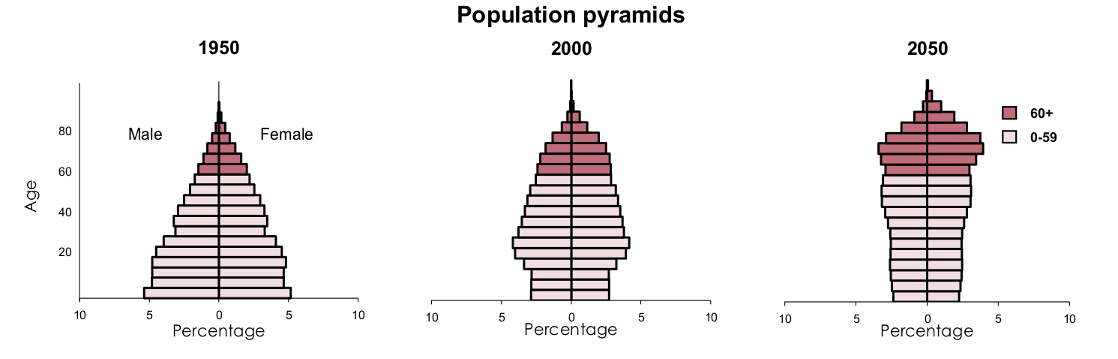
\includegraphics[width=1\textwidth]{img/01_demografia_pt.png}
  \caption{An�lise e previs�o da popula��o em Portugal entre 1950-2050. \cite{1}}
  \label{fig:cap1:demogPT}
\end{figure}

Pessoas com defici�ncias f�sicas ou mentais apresentam tamb�m uma id�ntica necessidade de acompanhamento. Por exemplo, pessoas com defici�ncia mental m�dia, normalmente t�m capacidades sociais e funcionais para serem minimamente independentes, ainda que necessitem de alguma supervis�o e assist�ncia. Normalmente t�m problemas t�o b�sicos como, por exemplo, decidir quando se levantar ou deitar na cama, ou tomar medicamentos � hora certa.

A monitoriza��o de ambos os casos descritos permitiria libertar m�o-de-obra especializada para situa��es de maior depend�ncia, reduzindo custos e aumentando a efici�ncia, notificando m�dicos ou hospitais da mudan�a de sinais vitais que precedam situa��es de risco ou interagindo com ambientes inteligentes.

A evolu��o tecnol�gica dos sensores wireless tem vindo a introduzir no mercado sensores, r�dios e processadores de baixa pot�ncia e baixo custo. Estes dispositivos, com o seu reduzido tamanho, t�m um enorme potencial para o desenvolvimento de aplica��es centradas no utilizador. Com um vasto tipo de sensores, as aplica��es ub�quas\footnote{Aplica��o que tem como objectivo tornar a interac��o entre pessoa e m�quina invis�vel, integrando a inform�tica com ac��es e comportamentos naturais das pessoas.}   podem por isso surgir como alternativa de baixo custo e enorme valor acrescentado para monitoriza��o de pessoas num ambiente dom�stico, criando uma simbiose entre pessoa e m�quina que permita usufruir do direito de viver de forma independente, com privacidade, dignidade e total controlo da pr�pria vida.


\section{Objectivos}
\label{sec��o:introdu��o:objectivos}
Nesta disserta��o � proposto o desenvolvimento de uma solu��o onde uma ou mais pessoas, portadoras de um n� wireless, se movimentam num ambiente onde existem outros n�s wireless. Dever� ser poss�vel localizar cada pessoa e estabelecer uma comunica��o bidireccional entre esta e um servidor central. 

Assim definem-se os seguintes objectivos:
\begin{itemize}
	\item Identificar necessidades num ambiente dom�stico e propor para estas solu��es de hardware existentes no mercado;
	\item Definir a arquitectura do sistema e os papeis de cada interveniente;
	\item Identificar uma plataforma de simula��o existente que permita, de uma forma realista, simular o comportamento do sistema;
	\item Implementar a simula��o de um algoritmo de encaminhamento;
	\item Implementar a simula��o de um algoritmo de localiza��o;
	\item Analisar a simula��o com m�tricas que permitam conhecer o erro de localiza��o, bem como os limites e valores �ptimos do sistema;
\end{itemize}


\section{Principais Contribui��es}
\label{sec��o:introdu��o:contribui��es}
(a escrever no fim)

\section{Organiza��o da Disserta��o}
\label{sec��o:introdu��o:organiza��o}
(a escrever no fim)
%Esta disserta��o encontra-se organizada nos seguintes seis cap�tulos:
%\begin{enumerate}
%	\item \nameref{cap�tulo:introdu��o}
%	\item \nameref{chap:ea}
%	\item \nameref{chap:conclusoes}
%\end{enumerate}
%
%O \autoref{cap�tulo:introdu��o} inclui a introdu��o ao projecto, assim como os seus objectivos, contribui��es do trabalho desenvolvido e a presente explica��o da organiza��o da disserta��o.
%
%O \autoref{chap:ea} ...
%
%Finalmente, no \autoref{chap:conclusoes} s�o tiradas as conclus�es do trabalho efectuado, fazendo-se tamb�m refer�ncias ao trabalho futuro que pode ser feito sobre o apresentado nesta disserta��o.

\cleardoublepage


% %%%%%%%%%%%%%%%%%%%%%%%%%%%%%%%%%%%%%%%%%%%%%%%%%%%%%%%%%%%%%%%%%%%%%%
% Literature Review
% %%%%%%%%%%%%%%%%%%%%%%%%%%%%%%%%%%%%%%%%%%%%%%%%%%%%%%%%%%%%%%%%%%%%%%
\fancychapter{Estado da Arte}
\label{chap:2}

A gera��o actual de casas inteligentes tem tido uma maior evolu��o na intelig�ncia artificial do sistema central, em detrimento dos sistemas de monitoriza��o e controlo. A casa inteligente actual consiste em v�rios electrodom�sticos e outros dispositivos, com sensores, actuadores e/ou monitores biom�dicos, usados pelos residentes numa base di�ria. Em alguns casos a casa � monitorizada recorrendo a tecnologias �udio e v�deo, sendo que estes sistemas apresentam uma excelente forma de monitoriza��o mas t�m algumas desvantagens:

\begin{itemize}
\item Custos elevados devido ao uso de sensores sofisticados e equipamentos �udio-visuais;
\item Custos elevados de instala��o devido � instala��o individualizada;
\item Elevada largura de banda necess�ria;
\item Demasiada intrus�o no quotidiano da pessoa criando um sentimento de falta de privacidade ou desconforto.
\end{itemize}

Tr�s grupos de tecnologias emergem por entre a bibliografia revista:

\begin{itemize}
\item Monitoriza��o com Sinal V�deo ou �udio;
\item Monitoriza��o com Sensores \textit{Wearable};
\item Monitoriza��o com Sensores Dom�sticos.
\end{itemize}

\section{Monitoriza��o com Sinal V�deo ou �udio}
\label{chap:2:sec:1}
Em \cite{2} atrav�s de um sensor wireless equipado com um aceler�metro e transportado pela pessoa, s�o detectadas poss�veis quedas. Por forma a minimizar o n�mero de falsos alarmes, s�o usadas c�maras que cobrem o espa�o, que analisam a posi��o da pessoa e s�o activadas de acordo com a localiza��o do n� m�vel. Essa localiza��o � obtida atrav�s de triangula��o baseada nas posi��es conhecidas dos n�s fixos e a pot�ncia recebida do n� m�vel. � tamb�m apresentada a possibilidade de efectuar transmiss�o de voz utilizando o r�dio IEEE 802.15.4, uma vez que j� existem r�dios com largura de banda necess�ria para efectuar transmiss�o de voz.

\begin{figure}[!htb]
  \centering
  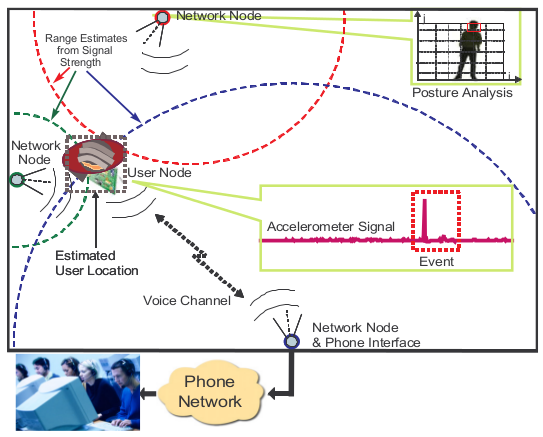
\includegraphics[width=0.65\textwidth]{img/02_video_monit_01.png}
  \caption{Arquitectura do sistema proposto em \cite{2}.}
  \label{fig:1:video_monit_01}
\end{figure}

Em \cite{3} e \cite{4} � feita a combina��o da informa��o fornecida por redes de sensores e sistemas de v�deo-vigil�ncia. Atrav�s de uma infer�ncia l�gica que considera sequ�ncias de eventos s�o tomadas decis�es tal como � poss�vel observar em \ref{fig:2:video_monit_02}. O ocupante da casa usa um sensor n�o intrusivo para determina��o da posi��o e comunica��o por voz, mas n�o � necess�ria qualquer interac��o com a tecnologia. � semelhan�a do trabalho anterior a privacidade � um tema fulcral e todo o tratamento de imagem � feito localmente usando \textit{Smart Cameras} \footnote{c�maras que para al�m de captar imagem tamb�m podem tratar a imagem e obter resultados a partir desta}.

\begin{figure}[!htb]
  \centering
  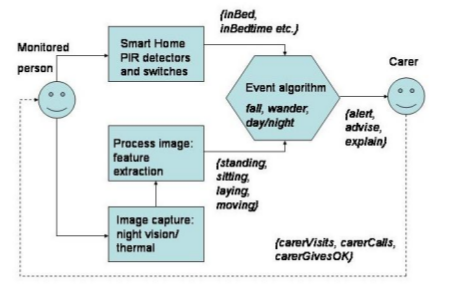
\includegraphics[width=0.75\textwidth]{img/02_video_monit_02.png}
  \caption{Arquitectura de fus�o de decis�o referida em \cite{3}.}
  \label{fig:2:video_monit_02}
\end{figure}

No trabalho \cite{5} � feita a aplica��o de um sistema de monitoriza��o num lar de idosos atrav�s de v�deo e �udio sem recurso a sensores port�teis. O trabalho referencia a insufici�ncia de profissionais em contraste com o r�pido crescimento da popula��o idosa e o pouco tempo que estes t�m dispon�vel para cada idoso. Emerge assim a necessidade de obter um conjunto de dados de forma aut�noma e usado para detectar situa��es de perigo de atempadamente, como por exemplo a instabilidade do andar ou registos comportamentais que favorecem a prescri��o de medicamentos psicotr�picos. Os grandes desafios indicados s�o a localiza��o por v�deo, a correcta identifica��o e marca��o das pessoas no campo de vis�o e a an�lise das suas actividades individuais.

Partindo do conceito \textit{aging in place}, onde idosos vivem de forma independente e segura nas suas pr�prias casas, o trabalho \cite{6} apresenta, a monitoriza��o de quedas mas tamb�m funcionalidades utilit�rias como a detec��o de objectos, calend�rio, v�deo-confer�ncia e livro de endere�os. Recorrendo a c�maras e a t�cnicas de \textit{machine learning} o sistema n�o necessita que o utilizador use um sensor. O sistema tem uma abordagem centralizada devido � forte exig�ncia de processamento em tempo real e mem�ria necess�rias. A detec��o de objectos � feita verificando mudan�as na imagem ou procurando objectos de acordo com as suas caracter�sticas. 

\begin{figure}[!htb]
  \centering
  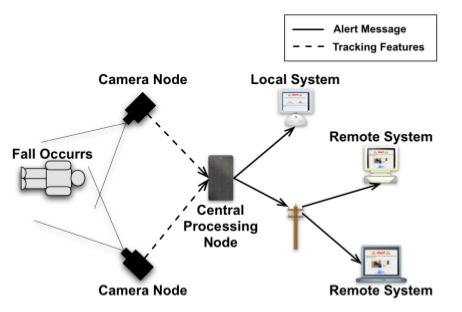
\includegraphics[width=0.8\textwidth]{img/02_video_monit_03.png}
  \caption{Processo de detec��o de quedas e alertas descrito no trabalho \cite{6}.}
  \label{fig:3:video_monit_03}
\end{figure}

Em \cite{7} � utilizado o sinal �udio em conjunto com o v�deo para inferir acerca de uma poss�vel queda. O sinal �udio torna-se essencial para distinguir entre uma pessoa que se sentou ou que caiu. Consideram-se processos de textit{Markov}\footnote{Processo sem mem�ria onde podem ser feitas previs�es do futuro com base somente no estado presente, onde o futuro � independente do passado} que permitem perceber se o comportamento do indiv�duo est� de acordo com o previsto ou n�o e assim tomar as medidas necess�rias.

Embora cada aplica��o tenha as suas mais-valias e a precis�o dos sistemas onde o sinal v�deo � utilizado seja bastante elevada, existe a quest�o da privacidade que resulta numa baixa aceita��o deste tipo de sistemas por parte de pessoas idosas.

A grande preocupa��o nos trabalhos identificados permanece na detec��o de quedas e na fiabilidade dessa detec��o.

\section{Monitoriza��o com Sensores \textit{Wearable}}
\label{chap:2:sec:2}
Com a evolu��o dos sensores wireless aparecem cada vez mais solu��es que permitem fazer uma monitoriza��o cont�nua do estado de sa�de de uma pessoa, independentemente da sua localiza��o ou actividade. A redu��o do tamanho dos sensores permite idealizar a cria��o de vestu�rio com sensores embutidos, suficiente leve e confort�vel para poder ser usado diariamente. Para al�m da monitoriza��o h� tamb�m a possibilidade de administrar medicamentos, recorrendo a actuadores, automaticamente ou de forma manual por um profissional de sa�de de forma remota.

Em \cite{8} � abordada a \acs{BSN}(\textit{Body Sensor Network}) como solu��o para a detec��o precoce de problemas card�acos. Atrav�s de um conjunto de sensores equipados com medidor de temperatura, medidor de pulso, aceler�metro e at� sensores capazes de obter um electrocardiograma\footnote{Representa��o gr�fica da actividade el�ctrica do cora��o} (ECG), um electromiograma\footnote{Representa��o do potencial el�ctrico gerado pelas c�lulas dos m�sculos} (EMG) ou um electroencefalograma\footnote{Representa��o da actividade do c�rebro, obtida por pequenos sinais el�ctricos chamados impulsos} (EEG). O sistema abordado tem um n� coordenador para onde todos os outros enviam informa��o e � usada a norma IEEE 802.15.4, que com suficiente largura de banda permite a transmiss�o da informa��o necess�ria.

\begin{figure}[!htb]
  \centering
  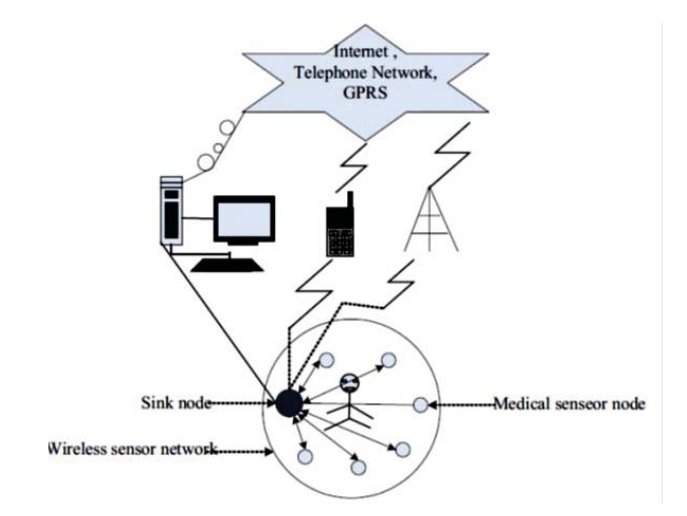
\includegraphics[width=0.5\textwidth]{img/02_body_sensor_network.png}
  \caption{Exemplo de uma \acs{BSN} \cite{8}.}
  \label{fig:4:bsn}
\end{figure}

A aplica��o corre em TinyOS, open-source e com uma gest�o de energia eficiente.
� referida a estrutura modular do sistema operativo que permite escolher componentes conforme a sua aplica��o, o que facilita bastante a utiliza��o de diferentes tipos de sensores. 

De referir o grupo de estudo IEEE 802.15 TG6\footnote{http://www.ieee802.org/15/pub/TG6.html} que pretende estabelecer a norma para as \acs{BAN}s (\textit{Body Area Networks}), que define um protocolo de comunica��o para dispositivos de baixa pot�ncia que operem dentro, em ou � volta do corpo humano.

Em \cite{9} � feita uma discuss�o sobre o tipo de antena e protocolo \acs{MAC} para \acs{WBAN}s, bem como sobre diversas aplica��es para este tipo de redes. Na Figura \ref{fig:5:wban} podemos observar que o tr�fego � categorizado em 3 categorias: \textit{On-demand} iniciado pelo m�dico ou n� coordenador para obter uma determinada informa��o de um ou mais sensores, \textit{Emergency} iniciado pelos n�s quando ultrapassam um determinado \textit{threshold} e \textit{Normal} que n�o apresenta qualquer elemento temporal cr�tico. 

\begin{figure}[!htb]
  \centering
  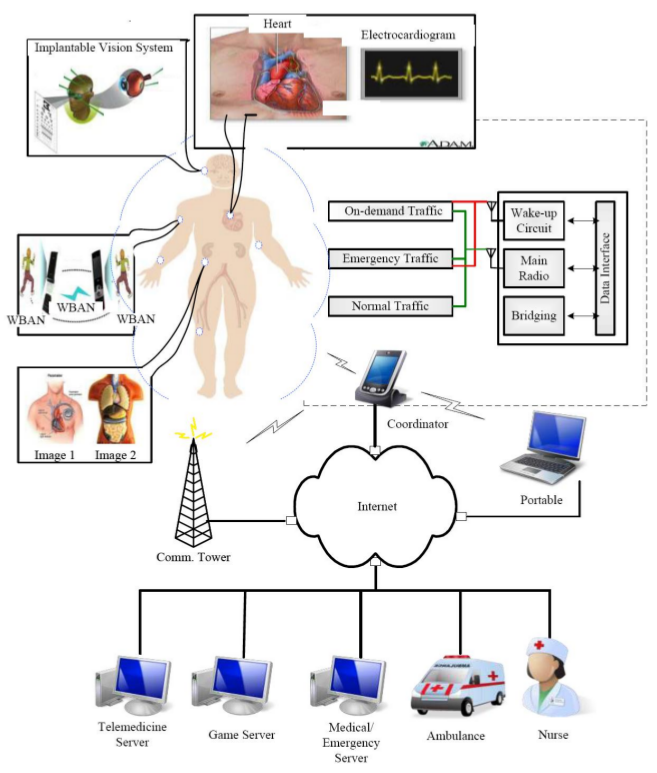
\includegraphics[width=0.80\textwidth]{img/02_wireless_body_area_network.png}
  \caption{Exemplo de uma \acs{WBAN} \cite{9}.}
  \label{fig:5:wban}
\end{figure}

� referido o impacto do corpo na propaga��o do sinal atrav�s da constante diel�ctrica alta que este possui bem como atrav�s da condutividade parcial do tecido muscular que pode absorver parte do sinal, factores que se tornam ainda mais significativos quando as antenas s�o de muito pequena dimens�o. Outro aspecto relevante referido neste trabalho � o facto de n�o existir no IEEE 802.15.4 um mecanismo fi�vel para o envio das mensagens \textit{On-demand} e \textit{Emergency}. Como poss�vel solu��o para este problema � apontada a utiliza��o das IEEE 802.15.4 \acs{GTS}(Guaranteed Time Slots) para lidar com eventos cr�ticos.

Por fim, o trabalho \cite{9} indica atrav�s da Tabela \ref{tab:1:sensor_apps} um conjunto de poss�veis aplica��es para sensores. Doen�as cardiovasculares, detec��o de doen�as oncol�gicas, sistemas de tele-medicina s�o algumas das aplica��es mencionadas.

\begin{table}
	\centering
	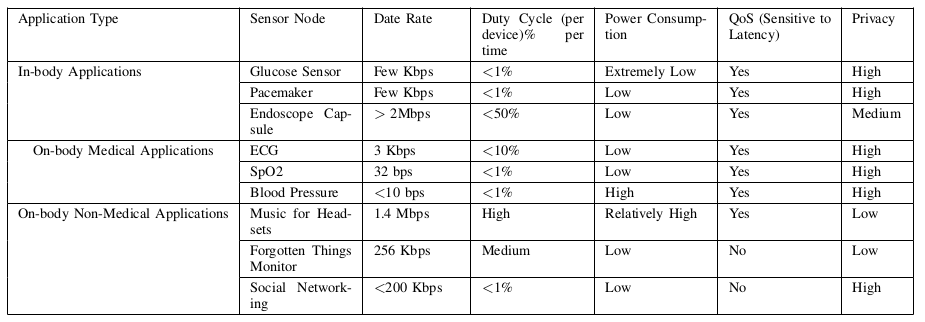
\includegraphics[width=1\textwidth]{img/02_inbody_onbody_applications.png}
  \caption{Aplica��es para redes de sensores \textit{In-body} e \textit{On-body} \cite{9}.}
  \label{tab:1:sensor_apps}
\end{table}

No trabalho \cite{10} � analisada a coexist�ncia entre \acs{WLAN} e \textit{ZigBee} que operam na mesma frequ�ncia de 2.4GHz. A problem�tica de um n�mero elevado de m�dulos \acs{WLAN}, com pot�ncia de transmiss�o mais elevada,  impossibilitar a comunica��o entre m�dulos \textit{ZigBee} � abordada. � sugerida como solu��o a implementa��o de um algoritmo implementado na \acs{WSN} que for�a a que, quando n�o existem frequ�ncias dispon�veis, a \acs{WLAN} seja obrigada a abandonar o canal deixando assim espa�o para o sistema \textit{ZigBee} comunicar. 

\cite{11} prop�e um projecto que integra tecnologias \acs{WSN} com redes p�blicas de comunica��o por forma a construir um sistema eficiente de cuidados de sa�de para idosos em casa. O sistema apresenta quatro funcionalidades principais: monitoriza��o interior, monitoriza��o exterior, actividade e decis�o com base no estado de sa�de. � feita a medi��o e colec��o de par�metros do corpo e da casa e enviada para um servidor central atrav�s de v�rias redes dispon�veis.

Uma das principais desvantagens abordada na pesquisa efectuada � o facto de ter de existir de forma cont�nua um contacto com o corpo do idoso, de v�rios sensores, o que pode causar desconforto. Muitos idosos poder�o n�o estar predispostos para usar uma \acs{BSN} durante um tempo prolongado. Existe tamb�m a possibilidade de interfer�ncia com \textit{pacemakers} ou outros equipamentos m�dicos que tenham sido colocados no idoso.

\section{Monitoriza��o com Sensores Dom�sticos}
\label{chap:2:sec:3}

Neste tipo de monitoriza��o recorre-se a sensores instalados em electrodom�sticos e outros dispositivos utilizados pelos residentes. S�o obtidos padr�es comportamentais atrav�s da correla��o com a utiliza��o dos diversos aparelhos numa casa. Uma das maiores vantagens deste tipo de monitoriza��o � a privacidade, uma vez que a informa��o fornecida por cada sensor n�o cont�m qualquer identifica��o da pessoa que o acciona. Usam-se dispositivos do dia-a-dia o que n�o implica mudan�as de comportamento, como por exemplo com a utiliza��o dos sensores \textit{Wearable} e as \acs{BSN}. Esta abordagem � chamada de \textit{artefact computing model} e representa um paradigma de mudan�a na interac��o pessoa-m�quina na sua forma expl�cita para uma forma impl�cita.

Identificam-se v�rios tipos de sensores aplic�veis a dispositivos dom�sticos:

\begin{itemize}
\item Sensores de press�o;
\item Sensores de movimento e proximidade;
\item Sensores de temperatura;
\item Sensores \acs{RFID};
\item Interruptores;
\item Sensores de vibra��o;
\item Sensores de caudal de �gua ou g�s;
\item Sensores de corrente;
\end{itemize}

No artigo \cite{15} aborda-se a presta��o de cuidados de sa�de aos idosos num complexo constru�do pela \textit{Elite Care}\footnote{http://www. elite-care.com}.Com o objectivo de dar maior autonomia aos residentes s�o criados ambientes personalizados de sensores. O sistema permite identificar residentes que precisam de cuidados imediatos ou iluminar o caminho para um residente que se v� durante a noite � casa-de-banho. A informa��o monitorizada neste sistema pertence a tr�s categorias: sinais vitais, sinais de entrada/sa�da e movimento. Na Tabela \ref{tab:2:pervasiveness}, a partir de um estudo feito com question�rios feitos aos residentes � obtido o grau de intrus�o de cada uma das tecnologias implementadas.

\begin{table}[!htb]
  \centering
  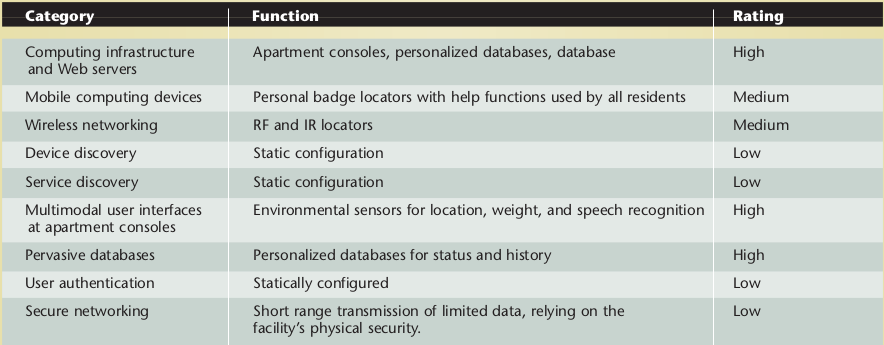
\includegraphics[width=1\textwidth]{img/02_grau_de_intrusao.png}
  \caption{Grau de intrus�o por tecnologia usada em \cite{15}.}
  \label{tab:2:pervasiveness}
\end{table}

\cite{13} usa sensores de press�o para localiza��o. � referida, a t�tulo de exemplo, a aplica��o do sistema a uma pessoa com doen�a de Alzheimer num est�dio m�dio e cuja detec��o do movimento permite activar ecr�s que se ligam quando a pessoa se aproxima e indicam as op��es de percurso na casa. Os melhores sensores conseguem identificar a posi��o e direc��o do utilizador, no entanto a \$10800 por metro quadrado n�o � uma alternativa vi�vel. No projecto s�o usados os \textit{Phidgets} 1.5 polegadas que para 32.5 metros quadrados custa \$4000. Sendo o custo uma desvantagem evidente s�o propostas alternativas, como por exemplo a redu��o de sensores �s zonas previs�veis de passagem ou a utiliza��o de modelos de previs�o que preencham as sec��es sem sensores.

Em \cite{14} � abordado o \textit{PlaceLab}. Situado em Cambrige � um laborat�rio vivo para estudo das tecnologias ub�quas. Est� optimizado para moradias 1 habitantes. Foram criadas para este laborat�rio 15 divis�es e em cada foram colocadas redes de 25 a 30 sensores. 

O projecto \textit{Mediacup} \cite{12} faz uma an�lise da adapta��o de sensores, processamento e comunica��o a dispositivos dom�sticos. Neste artigo uma caneca � adaptada com sensores de movimento e temperatura e ligada em rede com diversos outros dispositivos. Num cen�rio completo, todos os objectos de uso di�rio numa casa poderiam ser adaptados. � usado um processador de 1MHz para redu��o do consumo energ�tico e o carregamento feito usando um campo electromagn�tico instalado num pires. � utilizada a tecnologia \acs{IR} para a comunica��o, atrav�s de mensagens, com transdutores que usam uma arquitectura \acs{CAN}(Car Area Network) integrada por sua vez com uma \acs{LAN} (Figura \ref{fig:6:mediacup})

\begin{figure}[!htb]
  \centering
  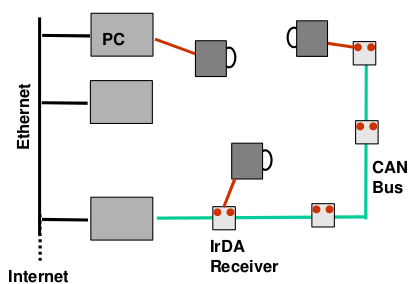
\includegraphics[width=0.75\textwidth]{img/02_mediacup.png}
  \caption{Infraestrutura de rede \textit{Mediacup} \cite{12} que integra \acs{IR}, \acs{CAN} e \acs{LAN}.}
  \label{fig:6:mediacup}
\end{figure}

% Ensure that the next chapter starts in a odd page
\cleardoublepage

% %%%%%%%%%%%%%%%%%%%%%%%%%%%%%%%%%%%%%%%%%%%%%%%%%%%%%%%%%%%%%%%%%%%%%%
% Literature Review
% %%%%%%%%%%%%%%%%%%%%%%%%%%%%%%%%%%%%%%%%%%%%%%%%%%%%%%%%%%%%%%%%%%%%%%
\fancychapter{Trabalho Relacionado}
\label{chap:3}

\section{Monitoriza��o Dom�stica de Idosos}
\label{chap:3:sec:2}
Em \cite{16} faz-se uma an�lise de aspectos fundamentais na monitoriza��o dom�stica de idosos ouvindo os profissionais de cuidados de sa�de. S�o tamb�m neste mesmo trabalho sugeridas diversas propriedades monitoriz�veis e feita uma an�lise global da rede de cuidados de sa�de.

\subsection{Necessidades nos Cuidados de Sa�de}
\label{chap:3:sec:2.1}

No estudo intitulado \textit{``The Activities of Daily Living Study''} em \cite{16} s�o examinados question�rios (91) feitos a profissionais de sa�de que prestam cuidados de monitoriza��o ao domic�lio. Pretende-se determinar a forma como a tecnologia pode ajudar pessoas idosas a envelhecer em casa, tendo em conta os profissionais de sa�de, a necessidade de autonomia do idoso e as necessidades da fam�lia e amigos.

Designam-se \acfp{CM} aos profissionais de sa�de que prestam cuidados ao domic�lio (ex:enfermeiros,m�dicos). Os \acs{CM}s interagem de forma activa com as pessoas idosas presencialmente ou por telefone. Avaliam a habilidade do idoso e a sua predisposi��o para a introdu��o de novos equipamentos. Uma parte significativa da monitoriza��o do \acs{CM} s�o as chamadas \acfp{ADL}, uma lista de actividades que permite medir a fun��o cognitiva e f�sica do idoso (Tabela \ref{tab:1:adls}).

\begin{table}[!htb]
  \centering
  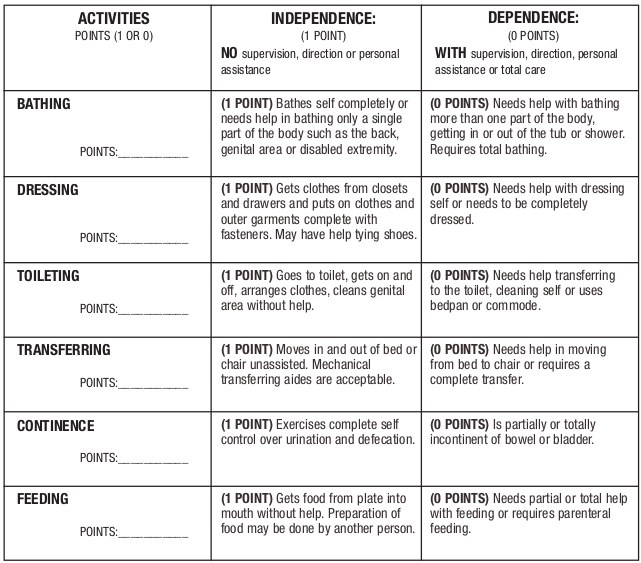
\includegraphics[width=1\textwidth]{img/03_adls.png}
  \caption{�ndice de independ�ncia nas \acs{ADL}s \cite{17}.}
  \label{tab:1:adls}
\end{table}

Esta lista permite definir numa escala de 0-muito dependente a 6-independente, o grau de depend�ncia do idoso. S�o tamb�m apresentados desafios � introdu��o de novas tecnologias pelos \acs{CM}s, nomeadamente:

\begin{itemize}
\item Receio de perda do emprego por parte dos \acs{CM}s;
\item Problemas de aceita��o da nova tecnologia por parte dos idosos, visto que estes t�m tend�ncia a esconder informa��o com receio de irem para a um lar de idosos;
\item Problemas de privacidade;
\end{itemize}

O processo de integra��o de um sistema de monitoriza��o apenas pode ser um sucesso se os profissionais de sa�de estiverem activamente envolvidos na sua implementa��o.

S�o identificadas diversos problemas de sa�de nos idosos, sendo os mais comuns a fraqueza, diabetes, surdez, perda de vis�o, defici�ncia nutricional e dem�ncia moderada.

\begin{table}[!htb]
  \centering
  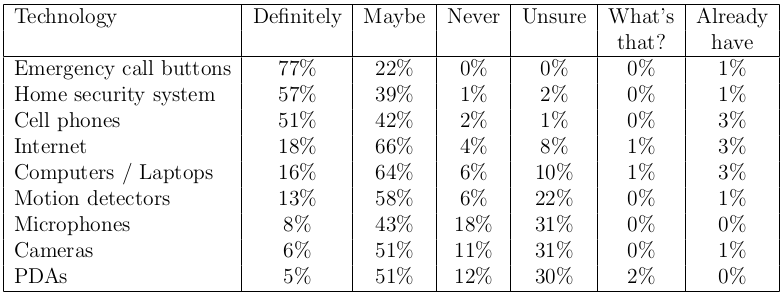
\includegraphics[width=0.95\textwidth]{img/03_elder_tech_acceptance.png}
  \caption{Uso de tecnologia pelos Idosos \cite{16}.}
  \label{tab:3:elderTechAccept}
\end{table}

Na Tabela \ref{tab:3:elderTechAccept} o estudo identifica as tecnologias e a sua aceita��o por parte dos idosos. A comunica��o e a seguran�a s�o identificados claramente como muito valorizados, atrav�s dos bot�es de emerg�ncia e sistemas de seguran�a, enquanto que a tecnologia de monitoriza��o coloca mais incerteza e desconfian�a aos idosos. 

\subsection{Necessidades na Monitoriza��o}
\label{chap:3:sec:2.2}

Com base nos resultados do estudo referenciado na Sec��o \ref{chap:3:sec:2.1} o trabalho \cite{16} faz uma an�lise de diversas tem�ticas de utiliza��o de um sistema de monitoriza��o. 

\textbf{Localiza��o dom�stica}. Determinar se o idoso se levantou pela manh� e os seus padr�es de movimento s�o tamb�m apontadas como duas informa��es importantes. Uma granularidade menor que a divis�o pode por isso ser importante sendo necess�ria uma maior precis�o do sistema. 

\textbf{Agendamento de visitas ao domic�lio}. Saber se o idoso est� ou n�o em casa � apontado pelos \acs{CM}s como um factor de melhoria no agendamento de visitas ao domic�lio.

\textbf{Visitas ao Hospital e Socializa��o}. A integra��o do sistema de monitoriza��o dom�stico com outro baseado em GPS e integrado no sistema de sa�de permitiria para todos os intervenientes no sistema saber onde estava um idoso a qualquer momento para al�m do ambiente dom�stico.

\textbf{N�mero de ocupantes da casa}. Sabendo os padr�es de ocupa��o da casa � poss�vel perceber quais os momentos em que os idosos t�m menos apoio familiar. Em casos mais agudos esta monitoriza��o permitiria determinar se era ou n�o seguro para o idoso continuar em sua casa durante uma determinada altura do dia.

\textbf{Animais de estima��o}. A maioria dos clientes dos \acs{CM}s entrevistados tinham animais de estima��o o que pode ser um problema para sistemas baseados em sensores de press�o.

\textbf{Oportunidades de instrumenta��o}. S�o apresentadas diversas oportunidades de instrumenta��o sem grande necessidade da mudan�a de h�bitos como a aplica��o de sensores a bengalas, andarilhos ou cadeiras de rodas. O facto de existir uma baixa partilha deste tipo de objectos indica que seriam uma boa hip�tese de monitoriza��o n�o-intrusiva. 

\textbf{Privacidade}. � bastante refutada a utiliza��o de c�maras, microfones ou \acs{PDA}s enquanto que os sensores de movimento poderiam ser alternativas vi�veis.

\begin{table}[!htb]
  \centering
  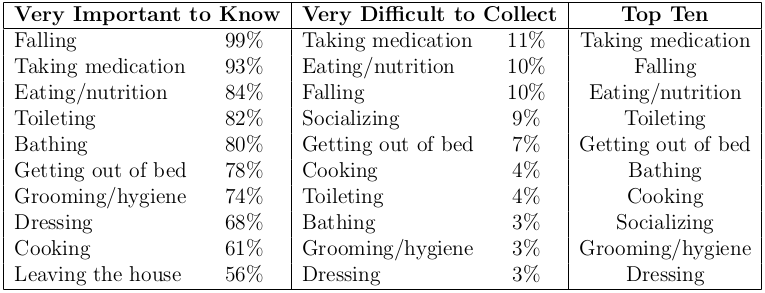
\includegraphics[width=0.9\textwidth]{img/03_adls_monit_rank.png}
  \caption{Classifica��o das \acs{ADL}s por import�ncia, dificuldade em monitorizar e top 10 das mais �teis \cite{16}.}
  \label{tab:4:adlsMonitRank}
\end{table}

\textbf{Escolha das \acs{ADL}s a monitorizar}. Na Tabela \ref{tab:4:adlsMonitRank} � feita uma classifica��o das \acs{ADL}s. O maior valor acrescentado est� naquelas que s�o mais dif�ceis de obter mas mais importantes para serem conhecidas pelo \acs{CM}.

\textbf{Aten��o � actividade das fam�lias ou assistentes}. � importante perceber se existe de facto um apoio real dos familiares ou outros assistentes ao idoso, para al�m de saber que o mesmo est� acompanhado.

\textbf{Monitoriza��o do uso de equipamentos}. A inclus�o nos equipamentos de sa�de de sensores que analisem o estado do equipamento ou a for�a exercida pelo idoso no mesmo, poderiam ajudar a determinar melhor o ponto em que � necess�rio passar de uma bengala para um andarilho ou de um andarilho para uma cadeira de rodas.

\section{Localiza��o em Redes de Sensores Wireless}
\label{chap:3:sec:3}
A chave para obter uma localiza��o fi�vel � representar de forma precisa os efeitos da degrada��o causada pelo canal de propaga��o no sinal. A propaga��o no mundo real sofre diversas perturba��es causadas por obstru��es, reflex�es e pessoas ou objectos em movimento, o que torna esta representa��o um problema de elevada complexidade. Nesta sec��o enumeram-se o tipo de medi��es que permitem inferir uma localiza��o e analisa-se bibliografia relacionada com o objectivo identificar algoritmos de localiza��o distintos, as suas vantagens e desvantagens na aplica��o ao objecto deste trabalho.

\subsection{Medidas de Localiza��o}
\label{chap:3:sec:3.1}
V�rios tipos de medi��es permitem inferir uma localiza��o, nomeadamente:

\begin{itemize}
\item \acs{TOA} (\textit{Time Of Arrival})
\item \acs{TDOA} (\textit{Time Difference Of Arrival})
\item \acs{RSS} (\textit{Received Signal Strength})
\item \acs{POA} (\textit{Phase Of Arrival})
\item \acs{AOA} (\textit{Angle Of Arrival})
\end{itemize}

Na medida do \textbf{\acs{TOA}} mede-se o tempo que um sinal demora a chegar ao n� de destino. A dist�ncia entre origem e destino � obtida multiplicando o atraso entre o momento da transmiss�o e o momento da recep��o do sinal pela velocidade de propaga��o do sinal.O requisito mais importante � a sincroniza��o entre n�s que obriga � exist�ncia de hardware de maior complexidade e a troca de mensagens de sincroniza��o. Ru�do aditivo e efeitos multi-caminho s�o as maiores fontes de erro neste tipo de medi��o.

Utilizando o \textbf{\acs{TDOA}} � medida a diferen�a entre os tempos de chegada em diversos n�s dum mesmo sinal enviado pelo emissor. Um m�nimo de dois n�s � necess�rio para uma estimativa em duas dimens�es da posi��o do do emissor. � semelhan�a do \acs{TOA} � necess�ria sincroniza��o entre os n�s o  que obriga uma vez mais a hardware complexo que aumenta o custo do n�.

O \acs{RSS} � a medida da pot�ncia do sinal recebido. Este m�todo n�o necessita de qualquer hardware especial para sincroniza��o. A pot�ncia do sinal � uma fun��o da dist�ncia, cuja localiza��o pode ser baseada num modelo, onde se admite que as caracter�sticas de propaga��o do sinal s�o bem conhecidas ou ent�o baseada num mapa de medi��es, \acs{RM} (\textit{Radio Map}), onde � feita uma amostragem da pot�ncia em diversas localiza��es.

Com a medida \acs{POA} o objecto de medi��o � o �ngulo de chegada. Este m�todo usa a diferen�a na fase do sinal para determinar a localiza��o do n� emissor.

Por �ltimo a medida de \acs{AOA} indica o �ngulo a que o sinal chega ao receptor, medido com antenas direccionais ou um conjunto de antenas.S�o usadas rela��es geom�tricas simples para calcular a posi��o do n� emissor.

\subsection{Algoritmos de Localiza��o}
\label{chap:3:sec:3.2}
Os esquemas de localiza��o s�o diversos e variam conforme o tipo de aplica��o. 

\begin{figure}[!htb]
  \centering
  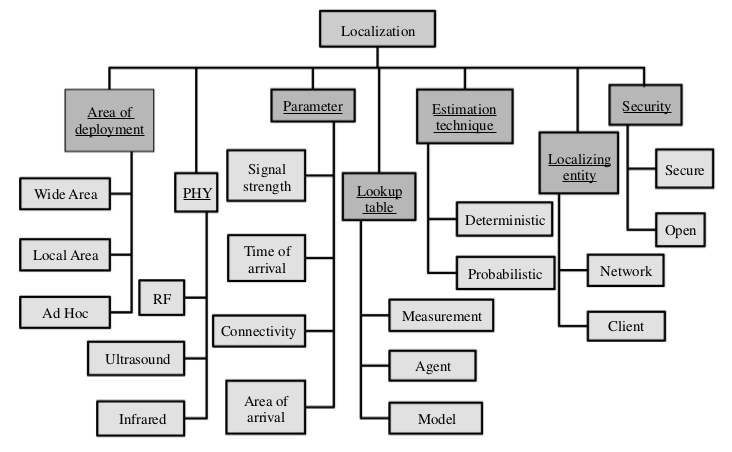
\includegraphics[width=1\textwidth]{img/03_localization_class.png}
  \caption{Classifica��o da localiza��o em redes \acs{WSN} \cite{27}.}
  \label{fig:3:localizationClass}
\end{figure}

A partir da Figura \ref{fig:3:localizationClass} � poss�vel fazer algumas observa��es relativas ao tema deste trabalho que permitir� reduzir a bibliografia a consultar.

\textbf{�rea de Instala��o}: A �rea de instala��o dever� ser local dado uma vez que estamos perante um ambiente dom�stico.

\textbf{PHY}: O meio de transmiss�o do sinal dever� ser a \acs{RF} (R�dio-Frequ�ncia) 

\section{Encaminhamento em Redes de Sensores Wireless}
\label{chap:3:sec:4}
Com a redu��o do custo dos sensores wireless tornou-se poss�vel construir \acs{WSN}s com centenas ou milhares de n�s. A falta de um esquema global de endere�amento, as condicionantes energ�ticas ou a possibilidade de existirem n�s que se movimentam provocando modifica��es na topologia da rede recorrentes, faz surgir a necessidade de encontrar um protocolo de encaminhamento adequado.

\subsection{Desafios e Decis�es de Design}
\label{chap:3:sec:4.1}
Em \cite{18} s�o abordados os diversos desafios no design de protocolos de encaminhamento.

Uma \acs{WSN} apresenta diversas restri��es tais como fornecimento de energia limitado pelo uso de bateria, processamento limitado ou largura de banda reduzida devido a r�dios relativamente simples.

\textbf{Instala��o dos n�s}. A forma como os n�s s�o instalados depende do tipo de aplica��o e pode ser determin�stica ou aleat�ria. Se for aleat�ria a distribui��o n�o � uniforme o que pode requerer \textit{clustering}. A dist�ncia de transmiss�o � reduzida o que obriga a que a comunica��o seja feita atrav�s de v�rios n�s.

\textbf{Toler�ncia a falhas}. Alguns sensores podem falhar devido � falta de energia, dano f�sico ou interfer�ncia. Essas falhas n�o podem por isso condicionar impedir a comunica��o e devem existir protocolos \acs{MAC} e de encaminhamento que consigam detectar essa situa��o e reformular a topologia da rede.

\textbf{Modelo de aquisi��o de dados}. A forma como � feita a aquisi��o de dados � dependente da aplica��o e pode ser orientada ao tempo, para aplica��es de monitoriza��o peri�dica ou ao evento para e � \textit{query}, para n�s que reagem a mudan�as na medi��o de par�metros ou a um pedido feito pela \acs{BS}. 

\textbf{Homogeneidade dos n�s ou liga��es}. Os n�s podem ter todos iguais capacidades sendo a rede homog�nea ou ent�o podem ter capacidades diferenciadas, havendo n�s mais b�sicos e outros mais complexos.

\textbf{Escalabilidade}. Devido ao elevado n�mero de n�s poss�vel numa \acs{WSN} qualquer protocolo de encaminhamento deve ser escal�vel reagindo de forma autom�tica � adi��o ou remo��o de n�s da rede.

\textbf{Din�mica da rede}. A maior parte das arquitecturas assume que os n�s est�o fixos. No entanto para aplica��es em que a topologia muda a estabilidade dos caminhos torna-se um assunto importante e algum tipo de actualiza��o peri�dica ou redescoberta de novos caminhos torna-se necess�rio.

\textbf{Agrega��o de dados}. Os dados de v�rios sensores podem ser agregados para que o n�mero de transmiss�es sofra uma redu��o. A agrega��o pode ser feita com remo��o de duplicados, valores m�nimos, valores m�ximos e valores m�dios. 

\textbf{\acs{QoS}} (\textit{Quality of Service}). Em algumas aplica��es os dados t�m de ser entregues com sucesso ap�s um determinado limite de tempo ap�s a sua obten��o, caso contr�rio perdem significado ou introduzem erros desnecess�rios no sistema. Este limite de tempo pode ser gerido de forma din�mica conforme a qualidade da transmiss�o.

\subsection{Protocolos de Encaminhamento}
\label{chap:3:sec:4.2}
Os protocolos nas \acs{WSN}s podem ser classificados conforme a sua estrutura em \textit{flat-routing} onde todos os n�s t�m as mesmas capacidades e pap�is na rede, \textit{hierarchical-routing} em que existem n�s com capacidades diferenciadas e pap�is diferentes e \textit{location-based routing} onde a posi��o dos n�s � parte integrante do protocolo de encaminhamento.

\title{\textbf{Flat-routing}}

O \acs{SPIN} (\textit{Sensor Protocols for Information via Negotiation}) \cite{20} surge com a necessidade de resolver tr�s problemas nos m�todos cl�ssicos de envio de mensagens (\textit{Flooding} e \textit{Gossiping}), a implos�o causada pela recep��o de v�rias mensagens repetidas vindas de v�rios n�s diferentes, a sobreposi��o resultante da dos dados obtidos por sensores pr�ximos e a falta de adapta��o aos recursos existentes no n�. Na Figura \ref{fig:1:spin} est� um exemplo onde s�o utilizadas os tr�s tipos de mensagens ADV (\textit{advertisment}), REQ (\textit{request} e DATA. O n� A pretende enviar uma mensagem para o n� B e envia um ADV (a). B est� pronto para receber e envia para A um REQ (b). A recebe o REQ e envia uma mensagem DATA para B (c). B continua o processo da mesma forma para os seus n�s vizinhos. Este protocolo permite poupar energia e reduzir o envio de informa��o redundante mas n�o d� garantias de entrega de dados.

\begin{figure}[!htb]
  \centering
  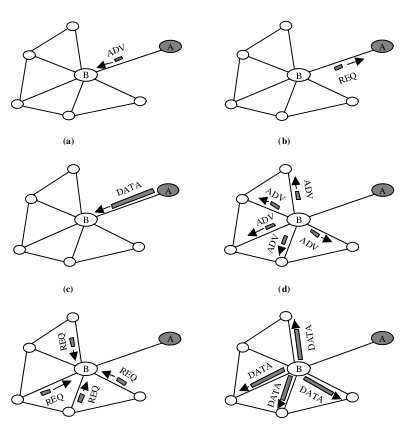
\includegraphics[width=0.85\textwidth]{img/03_spin.png}
  \caption{Protocolo \acs{SPIN} \cite{20}.}
  \label{fig:1:spin}
\end{figure}

O \acs{DD} (\textit{Direct Diffusion}) \cite{21}) introduz um m�todo de procura atrav�s da propaga��o de interesses e cria��o de gradientes constru�dos � medida que um determinado percurso vai sendo utilizado cada vez mais utilizado.

O \acs{AODV} (\textit{Ad hoc On-demand Vector Routing}) \cite{22} introduz o conceito da descoberta de caminhos e da persist�ncia dos mesmos de forma distribu�da por todos os n�s. � um protocolo \textit{On-demand} que s� entra em ac��o quando � necess�rio enviar uma nova mensagem e com mecanismos de \textit{Self-healing} que permitem recuperar um caminho quando por alguma raz�o existiu uma altera��o de topologia. Apresenta duas fases, uma de descoberta de caminho e outra de utiliza��o desse caminho.

Em \cite{23} � abordado o \acs{DSR} (\textit{Dynamic Source Routing}) semelhante ao \acs{AODV} tem como objectivo diminuir a largura de banda consumida pelas mensagens de controlo e necessidade de manuten��o atrav�s de \textit{beacons}. O percurso � guardado na mensagem e vai sendo actualizado � medida que, na fase de descoberta de caminho, esta vai passando em cada n�.

\title{\textbf{Hierarchical-routing}}

No trabalho \cite{24} � proposto o \acs{LEACH} (\textit{Low-Enegery Adaptive Clustering Hierarchy}), um protocolo baseado em \textit{clusters}, que usa coordena��o entre n�s e atrav�s de uma mudan�a aleat�ria do \textit{cluster-head} distribui de forma eficiente o consumo de energia  por todos os n�s. Este protocolo consegue reduzir o consumo de energia at� oito vezes menos que outros protocolos hier�rquicos. O facto dos n�s estarem agrupados em \textit{clusters} permite que a informa��o dos diversos n�s n�o coordenadores possa ser agregada antes de ser enviada para uma \acs{BS}. Como desvantagens tem o facto de n�o ser aplic�vel em redes de grande �rea, tem um \textit{overhead} extra de mensagens controlo e assume que todos os n�s iniciam o seu funcionamento com a mesma energia e que tanto um n� coordenador como um n� simples consumem a mesma energia. Na Figura \ref{fig:2:leach} est� um exemplo de aplica��o.

\begin{figure}[!htb]
  \centering
  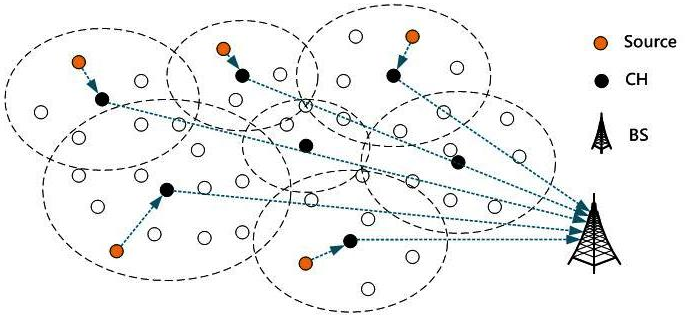
\includegraphics[width=1\textwidth]{img/03_leach.png}
  \caption{Exemplo de funcionamento do protocolo \acs{LEACH}.}
  \label{fig:2:leach}
\end{figure}

Outro protocolo hier�rquico � o \acs{PEGASIS} (\textit{Power-Efficient Gathering in Sensor Information Systems}) \cite{25} que surge como um melhoramento do \acs{LEACH}. Este protocolo aumenta o tempo de vida de cada n� usando t�cnicas colaborativas, onde cada n� fala apenas com o seu vizinho mais pr�ximo e transmite alternadamente para a \acs{BS}, eliminando assim a necessidade de forma��o de \textit{clusters} de forma din�mica e exist�ncia de v�rios n�s coordenadores. Como desvantagens o facto de se assumir que todos os n�s conseguem comunicar com a \acs{BS} directamente, que os n�s t�m o mesmo n�vel de energia e podem desligar-se ao mesmo tempo ou a possibilidade do coordenador �nico se tornar um \textit{bottleneck} no sistema.

\title{\textbf{Geographic-based Routing}}

Em \cite{26} � abordado o \acs{GEAR} (\textit{Geographical and Energy Aware Routing}). Este protocolo surge em redes com um n�mero elevado de sensores e onde poder�o ser feitas consultas a determinadas zonas geogr�ficas da rede, sem que tal seja feito com recurso a \textit{flooding}. S�o utilizadas heur�sticas baseadas na energia dos n�s e informa��o sobre a sua posi��o para encaminhar um pacote para uma determinar regi�o.

% Ensure that the next chapter starts in a odd page
\cleardoublepage

% %%%%%%%%%%%%%%%%%%%%%%%%%%%%%%%%%%%%%%%%%%%%%%%%%%%%%%%%%%%%%%%%%%%%%%
% State of the art
% %%%%%%%%%%%%%%%%%%%%%%%%%%%%%%%%%%%%%%%%%%%%%%%%%%%%%%%%%%%%%%%%%%%%%%

\fancychapter{Ambiente de Trabalho}
\label{chap:4}
As \acsp{WSN} s�o compostas por in�meros sensores wireless munidos de reduzidas capacidades de processamento, comunica��o e armazenamento. Antes da implementa��o de aplica��es que recorram a sensores wireless e respectiva arquitectura base (por exemplo, o TinyOS \cite{32}) em aplica��es reais, torna-se necess�rio avaliar a efici�ncia e robustez das mesmas, recorrendo a simula��es que englobem tanto a componente aplicacional do n� como a rede no seu todo. 

Nesta disserta��o sugere-se a cria��o de um ambiente de trabalho que resulta da utiliza��o conjunta de tr�s sistemas: a \acf{OMNeT++} \cite{33}, uma \textit{framework} base de simula��o por m�dulos,  o \acf{MiXiM} \cite{34}, uma uni�o de v�rias \textit{frameworks} para \acs{OMNeT++}, vocacionadas para a simula��o de sensores wireless e um componente de simula��o de obst�culos para o MiXiM \cite{35}.

\begin{figure}[!htb]
  \centering
  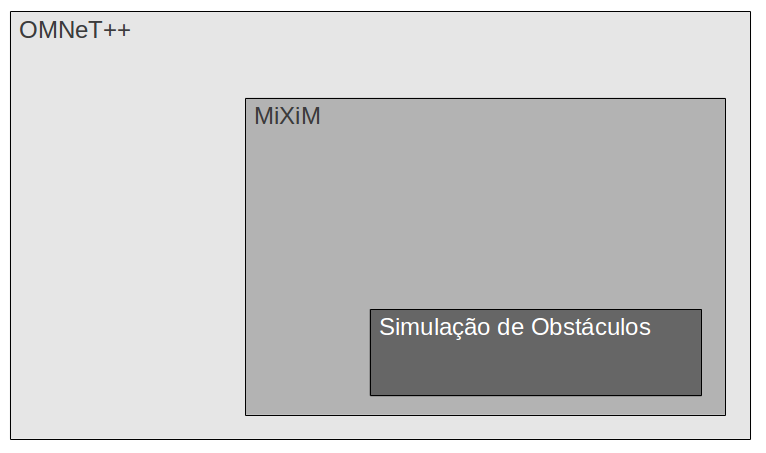
\includegraphics[width=0.70\textwidth]{img/04_framework_overview.png}
  \caption{Representa��o modular do ambiente de trabalho.}
  \label{fig:1:frameworkOverview}
\end{figure}

\section{Objective Modular network Test-bed (OMNeT++)}
\label{chap:4:sec:1}
O \acs{OMNeT++}\footnote{http://http://www.omnetpp.org/} � uma plataforma de simula��o baseada em m�dulos, escrita em C++ e com um IDE baseado em Eclipse. 

O \acs{OMNeT++} foi a plataforma base escolhida para este trabalho pelas seguintes raz�es:

\begin{itemize}
\item A partilha dos resultados deste trabalho com a comunidade \acs{OMNeT++}, promovendo a continuidade do trabalho efectuado nesta disserta��o;
\item A reutiliza��o e combina��o de m�dulos j� constru�dos;
\item A orienta��o por objectos que permite uma flex�vel extens�o das classes base;
\item A exist�ncia de um ambiente gr�fico autom�tico para uma melhor visualiza��o e \textit{debug} da simula��o;
\item A biblioteca extensa inclu�da que oferece suporte para estat�stica, colec��o de dados, apresenta��o gr�fica, n�meros aleat�rios e estruturas de dados;
\item A possibilidade simular v�rios cen�rios mudando apenas par�metros num ficheiro de configura��o, sem necessidade de nova compila��o.
\end{itemize}

Cada m�dulo pode ser do tipo simples ou composto. Os m�dulos compostos s�o constitu�dos por m�dulos simples ou por outros m�dulos compostos criando assim uma estrutura hier�rquica de depend�ncia.Todos os m�dulos assentam sobre um m�dulo de sistema, respons�vel pela realiza��o da simula��o. A comunica��o entre m�dulos � feita atrav�s do envio de mensagens, que podem ser t�o especializadas quanto o necess�rio, enviadas por canais de comunica��o de entrada e sa�da. Na Figura \ref{fig:2:omnet} est� um diagrama exemplificativo desta arquitectura.

\begin{figure}[!htb]
  \centering
  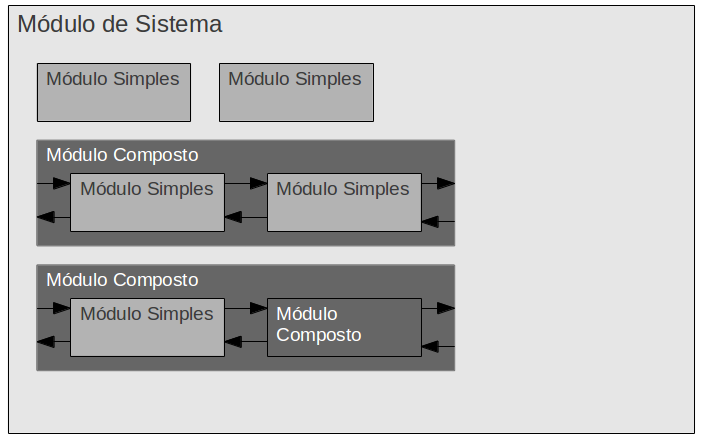
\includegraphics[width=0.80\textwidth]{img/04_omnet.png}
  \caption{Estrutura modular do OMNeT++.}
  \label{fig:2:omnet}
\end{figure}

A topologia de cada m�dulo e a forma como interliga com outros, � descrita utilizando a linguagem \acf{NED} sendo posteriormente a implementa��o feita em C++. � um utilizado um ficheiro de configura��o (ex: omnetpp.ini) que permite criar diversos cen�rios poss�veis definindo para cada um, por exemplo, par�metros dos m�dulos, tempo de simula��o, \textit{seed} para n�meros aleat�rios, etc. Esta solu��o permite a utiliza��o de apenas um execut�vel para diversas cen�rios.

Na Figura \ref{fig:3:omnetInternal} � poss�vel observar a estrutura interna de um execut�vel \acs{OMNeT++}.

\begin{figure}[!htb]
  \centering
  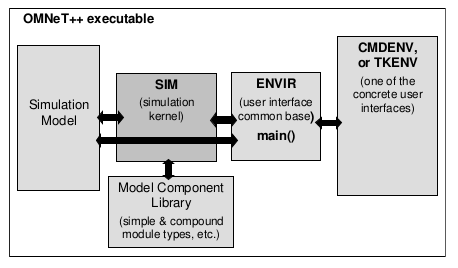
\includegraphics[width=0.85\textwidth]{img/04_omnet_internal.png}
  \caption{Arquitectura l�gica de um execut�vel OMNeT++ \cite{33}.}
  \label{fig:3:omnetInternal}
\end{figure}

A \textit{Model Component Library} cont�m o c�digo compilado dos m�dulos simples e compostos. Os m�dulos s�o instanciados e o \textit{Simulation Model} � constru�do pelo \textit{Simulation Kernel} (SIM) no in�cio da execu��o. A simula��o � ent�o executada num ambiente definido pelo utilizador que pode ser um dos disponibilizados no \acs{OMNeT++} (\textit{Tkenv} ou \textit{Cmdenv}) ou outro (ambiente criado pelo utilizador ou embebido noutra aplica��o). Para cada ambiente podem escolhidos ficheiros de configura��o (*.ini) e cen�rios definidos em cada ficheiro de configura��o. O ambiente \textit{Cmdenv} corre na linha de comandos de forma r�pida enquanto que o ambiente \textit{Tkenv} fornece um ambiente gr�fico capaz de animar de forma autom�tica o percurso das mensagens ou as posi��es dos n�s (Figura \ref{fig:4:omnetTkenv}).

\begin{figure}[!htb]
  \centering
  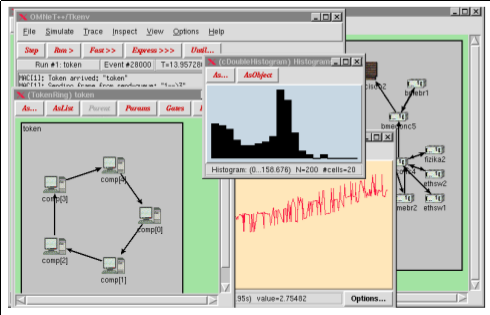
\includegraphics[width=1\textwidth]{img/04_omnet_tkenv.png}
  \caption{Ambiente de simula��o Tkenv no OMNeT++ \cite{33}.}
  \label{fig:4:omnetTkenv}
\end{figure}

\section{Mixed Simulator (MiXiM) para OMNeT++}
\label{chap:4:sec:2}
O \acs{MiXiM}\footnote{http://mixim.sourceforge.net/} resulta da combina��o de quatro \textit{frameworks}: a \acf{MF} que introduz suporte � mobilidade, o \acf{ChSim} que adiciona modelos detalhados de propaga��o, o MAC Simulator e a Positif Framework que adicionam o \acs{MAC}. Esta plataforma foi criada especificamente para simula��o de redes wireless introduzindo v�rias novidades �teis na simula��o de \acsp{WSN}, tais como:

\begin{itemize}
\item M�dulos para sensores wireless com diversas camadas e simula��o de bateria;
\item \acsp{NIC} de sensores wireless existentes no mercado (Texas Instruments CC1100 e CC2420);
\item Novos modelos de propaga��o de sinal, como por exemplo o \textit{Two-Ray Ground Path Loss} ou o \textit{Log-normal Shadowing};
\item A possibilidade de ter na mesma simula��o v�rios canais para diferentes frequ�ncias o que permite ter na mesma simula��o comunica��o WI-FI e \acs{GSM}.
\item A decis�o da qualidade do sinal e sua recep��o feita pelo n� receptor;
\item Novos m�dulos de mobilidade.
\end{itemize}

\begin{figure}[!htb]
  \centering
  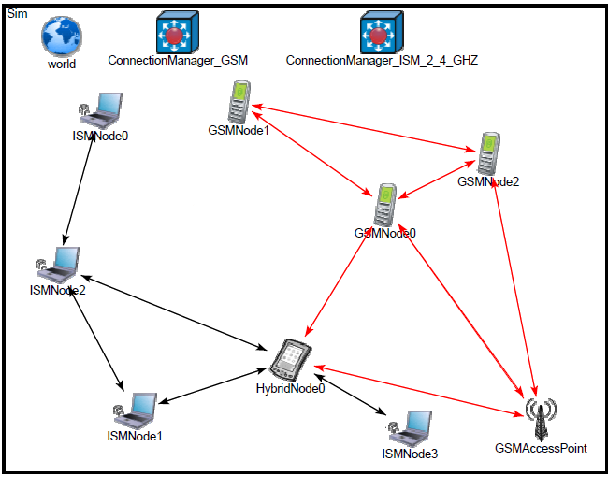
\includegraphics[width=0.85\textwidth]{img/04_mixim.png}
  \caption{Simula��o de uma rede no MiXiM \cite{34}.}
  \label{fig:5:mixim}
\end{figure}

Na Figura \ref{fig:5:mixim} temos a estrutura do \acs{MiXiM} que pode ser dividido em dois tipos de m�dulos:

\begin{itemize}
\item M�dulos de Simula��o: m�dulo \textit{world} respons�vel pela configura��o do ambiente (dimens�es da �rea de trabalho, gest�o de par�metros globais) e \textit{ConnectionManager} respons�vel pela gest�o das liga��es entre n�s. De notar que o MiXiM suporte v�rios n�s de liga��o, tantos como os canais de transmiss�o existentes;
\item M�dulos de N�: m�dulos com v�rios sub-m�dulos que implementam cada uma das camadas l�gicas e f�sicas presentes num n� de uma rede wireless.
\end{itemize}

\begin{figure}[!htb]
  \centering
  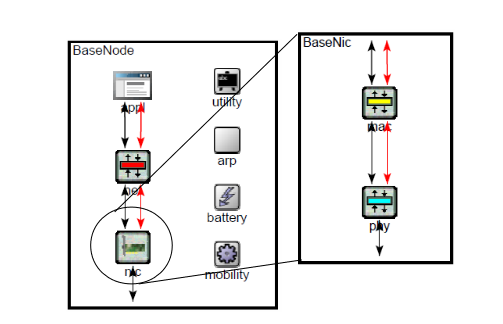
\includegraphics[width=0.70\textwidth]{img/04_mixim_node_module.png}
  \caption{M�dulo de n� no MiXiM \cite{34}.}
  \label{fig:6:miximNode}
\end{figure}

\begin{figure}[!htb]
  \centering
  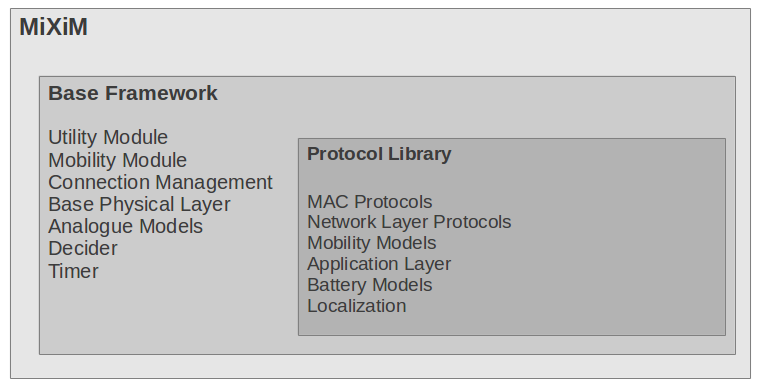
\includegraphics[width=0.85\textwidth]{img/04_mixim_logic_layers.png}
  \caption{Divis�o l�gica da \textit{framework} MiXiM.}
  \label{fig:7:miximLogicLayers}
\end{figure}

Na Figura \ref{fig:6:miximNode} observa-se em detalhe o m�dulo de n� onde est�o presentes as camadas l�gicas de um sensor wireless, o \acs{NIC} constitu�do pelas \acs{PHY} e \acs{MAC}, a camada \textit{Network} (Netw) e a camada de aplica��o. Existem ainda paralelamente v�rios sub-m�dulos, nomeadamente o \textit{mobility} que trata da posi��o e movimenta��o do n� na �rea de trabalho, o \textit{battery} que simula o consumo de energia, o \textit{arp} que trata do endere�amento e o \textit{utility} que serve para efeitos utilit�rios na partilha de informa��o durante a simula��o.

O \acs{MiXiM} pode ser dividido de forma l�gica numa plataforma base e numa biblioteca de protocolos conforme se pode observar na Figura \ref{fig:7:miximLogicLayers}. A plataforma base tem todos componentes necess�rios para criar uma simula��o. A biblioteca de protocolos tem diversas extens�es da plataforma base que permitem diversificar a quantidade de protocolos e modelos existente.

Importa analisar como funciona a camada \acs{PHY} no \acs{MiXiM}. A pot�ncia do sinal � influenciada pelo canal de propaga��o, influ�ncia que pode ser modelada por atenua��es causadas por efeitos de \textit{path loss}\footnote{Atenua��o causada pelo ar.}, \textit{shadowing}\footnote{Atenua��o causada por obst�culos.} e \textit{fading}\footnote{Atenua��o causada pela multi-propaga��o de um sinal derivada de diversas reflex�es.}. Para al�m disso tamb�m a frequ�ncia do sinal, a pot�ncia de envio e o \textit{bit-rate} (modula��o e codifica��o) no tempo, espa�o e frequ�ncia podem afectar a pot�ncia do sinal recebido.

Para modelar este complexo processo o MiXiM implementa uma classe especial de sinal que � associada a cada mensagem e implementa a camada \acs{PHY} tal como esquematizado na Figura \ref{fig:8:miximPhy}.

\begin{figure}[!htb]
  \centering
  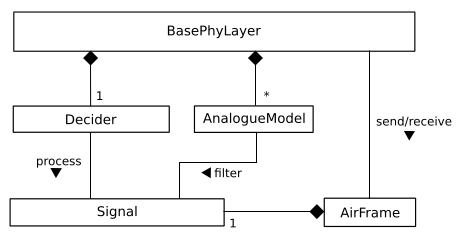
\includegraphics[width=0.75\textwidth]{img/04_mixim_phy.png}
  \caption{Camada PHY do MiXiM \cite{34}.}
  \label{fig:8:miximPhy}
\end{figure}

Quando recebe uma mensagem vinda do exterior (\textit{AirFrame}), a camada \acs{PHY} envia a mensagem para o modelo anal�gico que ir� calcular a atenua��o do sinal e para o \textit{Decider} que verifica se o sinal � ru�do com base na pot�ncia recebida e calcula os bit-errors. Depois deste momento a camada \acs{PHY} calcula o atraso de propaga��o e de transmiss�o da mensagem cabendo � camada \acs{MAC} determinar com base nos \textit{bit errors} se mensagem � v�lida ou n�o.


\section{Simula��o de Obst�culos para MiXiM}
\label{chap:4:sec:3}
Embora esteja referida em \cite{34}, a simula��o de obst�culos, como parte integrante do MiXiM, esta nunca chegou a ser implementada. Assim foi necess�rio procurar uma solu��o que permitisse simular a exist�ncia de obst�culos no ambiente de trabalho.

O trabalho \cite{35} implementa a simula��o de obst�culos no MiXiM e a sua representa��o no ambiente Tkenv. O modelo descrito n�o contempla efeitos de reflex�o ou difrac��o e pretende ser computacionalmente r�pido. A configura��o dos obst�culos � feita atrav�s de um ficheiro XML. Na \lstlistingname{} \ref{list:1:obstaclesXML} est� o c�digo XML necess�rio para desenhar o obst�culo da Figura \ref{fig:9:miximWithObstacles}.

\begin{workflow-code}{Exemplo de configura��o XML de obst�culos.}{list:1:obstaclesXML}
<obstacles>
   <poly id="wall#0" type="brickWall20cm" color="#F00" shape="12.8,10 13,10 13,15 12.8,15" />
</obstacles>
\end{workflow-code}

\begin{figure}[!htb]
  \centering
  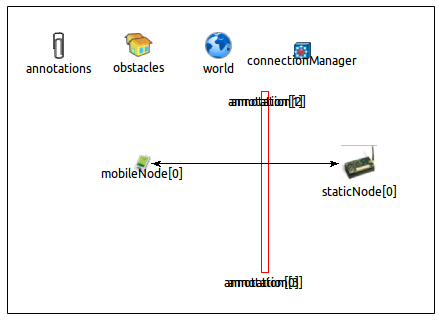
\includegraphics[width=0.75\textwidth]{img/04_mixim_with_obstacles.png}
  \caption{Simula��o de uma rede MiXiM com obst�culos.}
  \label{fig:9:miximWithObstacles}
\end{figure}


Para melhor perceber a solu��o encontrada analisa-se a base matem�tica do modelo.

Sabendo que a pot�ncia recebida de um sinal � dada por:

\begin{equation}
	P_r[dBm] = P_t[dBm] + G_t[dB] + G_r[dB] - \sum{L_x[dB]}
\end{equation}

onde \begin{math}P\end{math} � pot�ncia, \begin{math}G\end{math} � ganho e \begin{math}L_x\end{math} s�o os termos que traduzem as perdas. No MiXiM as perdas j� s�o calculadas como descrito na sec��o anterior pela camada \acs{PHY} mas n�o contemplam as perdas provocadas por obst�culos. 

� ent�o sugerido um termo para a pot�ncia provocada por obst�culos:

\begin{equation}
	L_{obs}[dB] = \beta{n} + \gamma{d_m}
\end{equation}

Os termos \begin{math}\beta{}\end{math} e \begin{math}\gamma{}\end{math} s�o calculados com base nos resultados obtidos experimentalmente e representam a atenua��o por metro e a atenua��o por parede respectivamente. Para o trabalho \cite{35} os valores obtidos foram \begin{math}\beta{}\approx{9dB}\end{math} e \begin{math}\gamma{}\approx{0.4dB/m}\end{math}. 

Devido � n�o utiliza��o de n�s reais neste trabalho, que permitissem chegar a valores reais, optou-se por considerar, com base no Tabela \ref{tab:1:attenuationPerInch} do manual da \textit{3Com Wireless Antenas}\footnote{http://www.scribd.com/doc/32613170/3Com\%C2\%AE-Wireless-Antennas}, os seguintes valores:

\begin{table}[!htb]
	\centering
\begin{tabular}{ |c|c|c|}
	\hline
  	Profundidade(cm) & \begin{math}\beta{}\end{math}(dBm)  & \begin{math}\gamma{}\end{math}(m)\\
  	\hline
  	20 & 106.3 & 0 \\
  	10 & 26.575 & 0 \\
  	\hline
\end{tabular}
	\caption{Valores de atenua��o por metro e por parede usados neste trabalho.}
	\label{tab:1:attenuationValues}
\end{table}

\begin{table}[!htb]
  \centering
  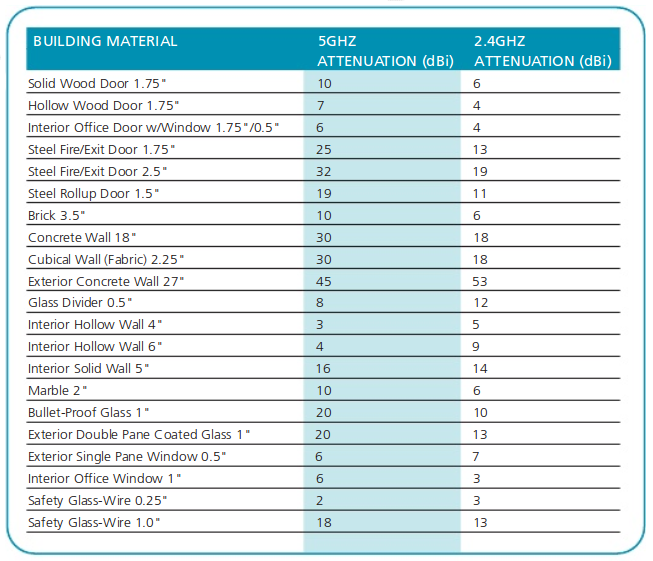
\includegraphics[width=1\textwidth]{img/04_attenuation_per_inch.png}
  \caption{Atenua��o de materiais de constru��o comuns para frequ�ncias de 5GHz e 2.4 GHz.}
  \label{tab:1:attenuationPerInch}
\end{table}




% Ensure that the next chapter starts in a odd page
\cleardoublepage

% %%%%%%%%%%%%%%%%%%%%%%%%%%%%%%%%%%%%%%%%%%%%%%%%%%%%%%%%%%%%%%%%%%%%%%
% State of the art
% %%%%%%%%%%%%%%%%%%%%%%%%%%%%%%%%%%%%%%%%%%%%%%%%%%%%%%%%%%%%%%%%%%%%%%

\fancychapter{Arquitectura do Sistema}
\label{chap:im}
Pequena introdu��o.

\section{Pressupostos e Estrutura}
\label{sec:im:sec1}
Limita��es da framework que v�o diferir da realidade;
Explica��o de todos os intervenientes no sistema: n�s m�veis, est�ticos e de base;
A forma como est�o interligados; A forma como � feita a escalabilidade e distin��o entre redes de andares diferentes;
O tipo de n�s presentes no sistema.

\section{Ficheiros XML de Configura��o}
\label{sec:im:sec2}
RadioMap; RadioMapClusters; Normal standard; Esquema com os diversos ficheiros;

\section{Network Layer}
\label{sec:im:sec3}
Tipos de mensagens da camada Netw e fluxogramas como a forma como essas mensagens s�o tratadas por cada tipo de n�;
Estruturas que fazem parte da camada Netw utilizadas; Exemplo com imagens do AODV a funcionar;
NetwToApplicationInfo para transportar informa��o acerca da pot�ncia do sinal;

\subsection{\textit{Ad hoc On-Demand Vector Routing}}
\label{chap:4:sec:4.1}

\section{Application Layer}
\label{sec:im:sec4}
Explica��o da mensagem HoHuT e a forma como � usada para transportar informa��o;
Explica��o do comportamento, por fluxograma, de cada um dos app layers da camada App;

\subsection{HORUS}
\label{chap:5:sec:5.1}

% Ensure that the next chapter starts in a odd page
\cleardoublepage

% %%%%%%%%%%%%%%%%%%%%%%%%%%%%%%%%%%%%%%%%%%%%%%%%%%%%%%%%%%%%%%%%%%%%%%
% State of the art
% %%%%%%%%%%%%%%%%%%%%%%%%%%%%%%%%%%%%%%%%%%%%%%%%%%%%%%%%%%%%%%%%%%%%%%

\fancychapter{Resultados}
\label{chap:6}

\section{Par�metros de Configura��o}
\label{chap:6:sec:1}

\section{Caso de Estudo 1}
\label{chap:6:sec:2}



% Ensure that the next chapter starts in a odd page
\cleardoublepage

% %%%%%%%%%%%%%%%%%%%%%%%%%%%%%%%%%%%%%%%%%%%%%%%%%%%%%%%%%%%%%%%%%%%%%%
% Conclusions
% %%%%%%%%%%%%%%%%%%%%%%%%%%%%%%%%%%%%%%%%%%%%%%%%%%%%%%%%%%%%%%%%%%%%%%

\fancychapter{Conclus�es e Trabalho Futuro}
\label{chap:7}

Com o intuito de obter uma simula��o o mais fidedigna poss�vel, foi necess�rio ao longo deste trabalho, encontrar solu��es que n�o se limitassem a simular um ou outro aspecto do problema, mas sim o conjunto completo, de funcionalidades do sistema proposto. 

Grande parte do problema ficou resolvido com o \acs{MiXiM}, no entanto foi necess�rio encontrar um protocolo de encaminhamento adequado e um sistema de localiza��o que conjuntamente, permitissem criar um sistema completamente funcional de monitoriza��o.

Este trabalho permitiu assim desenvolver uma solu��o simulada de um sistema de monitoriza��o de pessoas idosas, sem deixar de referenciar o hardware necess�rio e adquirir um conhecimento alargado do protocolo de encaminhamento \acs{AODV} e do sistema de localiza��o HORUS.

Futuramente poder� ser melhorado o protocolo de localiza��o para que deixe de ser necess�rio existir uma fase \textit{offline}, utilizando-se n�s fixos que saibam a sua pr�pria localiza��o e que com isso criem de forma autom�tica e peri�dica novos mapas r�dio sem a necessidade de interven��o.

Outra possibilidade interessante, seria implementar no n� m�vel um conjunto de camadas paralelo com r�dio bluetooth, ligando assim esse n� tamb�m a uma rede \acs{BSN} simulada, o que permitiria recriar no ambiente de trabalho eventos humanos que despoletassem mensagens, como aumento da temperatura ou batimento card�aco.

A melhoramento do modelo de obst�culos ou at� mesmo a utiliza��o de n�s reais que permitissem chegar aos par�metros do modelo utilizado, seria tamb�m uma possibilidade interessante de trabalho futuro.

% Ensure that the next chapter starts in a odd page
\cleardoublepage

% Add the Bibliography to the PDF table of contents (not the document table of contents)
\pdfbookmark[0]{Bibliografia}{bib}
% The bibliography style sheet
% \bibliographystyle{plain}
\bibliographystyle{IEEEtran}
% \bibliographystyle{apalike}
% \bibliographystyle{unsorted}
% The BiBTeX file
\bibliography{3_referencias-anexos/referencias}
\cleardoublepage

\appendix

% %%%%%%%%%%%%%%%%%%%%%%%%%%%%%%%%%%%%%%%%%%%%%%%%%%%%%%%%%%%%%%%%%%%%%%
% First appendix
% %%%%%%%%%%%%%%%%%%%%%%%%%%%%%%%%%%%%%%%%%%%%%%%%%%%%%%%%%%%%%%%%%%%%%%
\fancychapter{Ap�ndice 1 - Ficheiros XML de Configura��o}
\label{annex:a}

\fancychapter{Ap�ndice 1 - Ficheiros XML de Exemplo}
\label{annexA}

%XML CONFIG radio MAP
\begin{annex-code}{Exemplo de ficheiro XML de configura��o do mapa r�dio.}{list:a1:xmlRadioMap}
<?xml version="1.0" encoding="UTF-8"?><radioMap maxPositionPDFsSize="4">
  <position x="2" y="2">
    <staticNodePDF address="1000" mean="-6.86524" stdDev="-2.39173"/>
    <staticNodePDF address="1005" mean="-19.6319" stdDev="-15.9808"/>
    <staticNodePDF address="1001" mean="-21.0037" stdDev="-19.5426"/>
    <staticNodePDF address="1006" mean="-22.8628" stdDev="-19.3251"/>
  </position>
  <position x="4" y="2">
    <staticNodePDF address="1000" mean="-8.58641" stdDev="-7.49053"/>
    <staticNodePDF address="1006" mean="-18.8375" stdDev="-16.4028"/>
    <staticNodePDF address="1005" mean="-19.2409" stdDev="-17.7517"/>
    <staticNodePDF address="1001" mean="-19.2659" stdDev="-19.1632"/>
  </position>
  <position x="3" y="2">
    <staticNodePDF address="1000" mean="31.6669" stdDev="33.1443"/>
    <staticNodePDF address="1005" mean="-22.0094" stdDev="-19.9634"/>
    <staticNodePDF address="1006" mean="-22.8608" stdDev="-21.7965"/>
    <staticNodePDF address="1001" mean="-23.1735" stdDev="-21.8065"/>
  </position>
  <position x="6" y="2">
    <staticNodePDF address="1001" mean="-10.6905" stdDev="-6.60051"/>
    <staticNodePDF address="1000" mean="-15.8409" stdDev="-15.7502"/>
    <staticNodePDF address="1006" mean="-18.4932" stdDev="-17.3782"/>
    <staticNodePDF address="1005" mean="-19.1748" stdDev="-18.4118"/>
  </position>
  <position x="5" y="2">
    <staticNodePDF address="1000" mean="-13.661" stdDev="-11.7475"/>
    <staticNodePDF address="1001" mean="-15.1687" stdDev="-13.708"/>
    <staticNodePDF address="1006" mean="-23.314" stdDev="-20.5445"/>
    <staticNodePDF address="1005" mean="-23.8983" stdDev="-22.9379"/>
  </position>
  <position x="7" y="2">
    <staticNodePDF address="1001" mean="-9.56809" stdDev="-8.91176"/>
    <staticNodePDF address="1000" mean="-16.7335" stdDev="-15.6741"/>
    <staticNodePDF address="1006" mean="-17.5364" stdDev="-15.7507"/>
    <staticNodePDF address="1002" mean="-17.5544" stdDev="-15.1108"/>
  </position>
</radioMap>
\end{annex-code}

\begin{annex-code}{Exemplo de ficheiro XML de configura��o do m�dulo \textit{TurtleMobility} do MiXiM.}{list:a1:xmlTurtleMobility}
<movement>
	<set speed="10" angle="180"/>
	<repeat n="4">
		<forward d="50"/>
		<turn angle="90"/>
    </repeat>
    <repeat>
		<set speed="uniform(10,20)"/>
        <turn angle="uniform(-30,30)"/>
        <forward t="uniform(0.1,1)"/>
    </repeat>
</movement>
\end{annex-code}

\clearpage

\begin{annex-code}{Exemplo de ficheiro XML de configura��o de \textit{clusters} de posi��es.}{list:a1:xmlRadioMapCluster}
<?xml version="1.0" encoding="UTF-8"?>
<radioMapClusters clusterKeySize="1">
  <cluster>
    <clusterKey>
      <staticNode address="1001"/>
    </clusterKey>
    <position x="6" y="2"/>
    <position x="7" y="2"/>
    <position x="8" y="2"/>
    <position x="9" y="2"/>
    <position x="10" y="2"/>
    <position x="11" y="4"/>
    <position x="10" y="4"/>
    <position x="9" y="4"/>
    <position x="8" y="4"/>
    <position x="7" y="4"/>
    <position x="6" y="4"/>
    <position x="10" y="6"/>
  </cluster>
  <cluster>
    <clusterKey>
      <staticNode address="1000"/>
    </clusterKey>
    <position x="2" y="2"/>
    <position x="3" y="2"/>
    <position x="4" y="2"/>
    <position x="5" y="2"/>
    <position x="5" y="4"/>
    <position x="4" y="4"/>
    <position x="3" y="4"/>
    <position x="2" y="4"/>
    <position x="2" y="5"/>
    <position x="2" y="6"/>
    <position x="3" y="6"/>
  </cluster>
</radioMapClusters>
\end{annex-code}

\cleardoublepage

\end{document}
